
\documentclass[UTF8,12pt,oneside]{ctexbook}
\usepackage[a4paper,margin=2.5cm,headheight=15pt]{geometry}
\usepackage{amsmath,amssymb,bm}
\usepackage{graphicx}
\usepackage{booktabs,array,longtable,multirow,tabularx}
\usepackage{float}
\usepackage{enumitem}
\usepackage{caption,subcaption}
\usepackage{algorithm}
\usepackage{algpseudocode}
\usepackage{xcolor}
\usepackage{hyperref}
\usepackage{fancyhdr}
\usepackage{titlesec}
\usepackage{setspace}
\usepackage{indentfirst}
\usepackage{url}

\setlength{\parindent}{2em}
\setlength{\parskip}{0.25em}
\setstretch{1.30}
\captionsetup{font=small,labelfont=bf}
\hypersetup{colorlinks=true,linkcolor=black,urlcolor=blue,citecolor=black}
\renewcommand{\arraystretch}{1.25}

\definecolor{chapterblue}{RGB}{34,76,125}
\titleformat{\chapter}{\centering\Huge\bfseries\color{chapterblue}}{第\thechapter 章}{1em}{}
\titleformat{\section}{\Large\bfseries\color{chapterblue}}{\thesection}{0.8em}{}
\titleformat{\subsection}{\large\bfseries}{\thesubsection}{0.8em}{}
\titleformat{\subsubsection}{\normalsize\bfseries}{\thesubsubsection}{0.8em}{}

\pagestyle{fancy}
\fancyhf{}
\fancyhead[L]{第三章 \quad 天基计算网络协同资源分配}
\fancyhead[R]{BC-CTDE-MAPPO}
\fancyfoot[C]{\thepage}

\newcolumntype{Y}{>{\raggedright\arraybackslash}X}
\newcolumntype{C}[1]{>{\centering\arraybackslash}p{#1}}

%% 图像文件统一采用 3-new-x 命名，例如 images/3-new-1.png
\begin{document}

\begin{titlepage}
\centering
\vspace*{4.2cm}
{\zihao{0}\bfseries 第三章\par}
\vspace{1.0cm}
{\zihao{2}\bfseries 天基计算网络协同资源分配\par}
\vspace{2.0cm}
{\zihao{4}本章围绕天基网络去中心化条件下的协同资源分配问题展开，\par}
{\zihao{4}重点给出问题分析、博弈建模、区块链增强求解框架与实验验证。\par}
\vfill
{\zihao{-4}\today\par}
\end{titlepage}

\frontmatter
\tableofcontents
\mainmatter
\setcounter{chapter}{2}

\chapter{天基计算网络协同资源分配}
\label{chap:ch3}

随着天基计算网络的规模化部署，分布式资源协同调度已成为支撑在轨实时任务处理的核心瓶颈。在无全局中心协调者的去中心化环境中，异构计算节点受自身效用最大化的理性决策驱动，往往倾向于争抢高价值任务、回避低收益负载，进而引发“单节点最优、系统全局劣化”的公地悲剧困境。这一困境在节点能力高度异构、任务到达过程非平稳、星间链路带宽受限等多维复杂性的耦合叠加下进一步加剧，导致传统集中式优化方法与简单启发式策略均难以有效适配。

针对上述挑战，本章将系统层协同资源分配问题建模为多智能体马尔可夫博弈，在理论上刻画节点间竞争—合作并存的交互结构，并提出一种区块链增强的集中训练—分散执行（Centralized Training and Decentralized Execution, CTDE）多智能体强化学习框架。该框架以联盟链作为“公共博弈信息板”，在保障去中心化自治的同时，实现全局状态的可信共享与策略审计；在奖励机制层面，设计融合任务完成质量、系统公平性与信誉激励的三维混合奖励函数，引导自利节点在纳什均衡方向上趋近社会最优。本章通过多场景仿真实验，从收敛性、负载均衡、任务完成率及抗自私攻击能力等维度验证所提方法的有效性与鲁棒性，为后续章节中服务层与任务层的协同优化奠定系统层基础。与近年来卫星边缘计算中的多智能体卸载研究相比，本章更强调“可信共享 + 博弈求解 + 信誉治理”的统一闭环\cite{ref1,ref2,ref3}。



\section{引言}

随着低轨卫星互联网、在轨智能处理与星间协同计算的发展，天基计算网络正在从“以通信为主”的基础设施演化为“通信、计算、存储、智能处理一体化”的分布式服务平台。不同轨道层、不同载荷能力以及不同链路条件的卫星节点，通过时变星间链路构成动态互联的在轨计算网络，共同承担遥感影像预处理、目标检测、轨道态势分析、数据压缩转发、任务规划等多类任务。与传统“先回传、后处理”的地面中心化模式相比，这种在轨协同处理方式能够显著降低原始数据的大规模回传压力，缩短任务响应路径，并提高系统在时敏型任务下的自主运行能力。因此，系统是否能够对异构节点进行高效、可信、持续的协同资源分配，已成为影响网络整体服务能力的关键基础问题。

然而，天基计算网络与地面云边协同系统相比存在更加突出的资源受限性和环境不确定性。首先，卫星节点的计算能力、可用存储、剩余能量和热控条件天然受限，无法简单通过横向扩容方式缓解局部过载；其次，星间链路的建立与维持高度依赖可见关系、轨道位置和瞬时拥塞状态，导致网络拓扑和通信条件持续变化；再次，任务负载并非平稳到达，不同类型任务在计算量、数据规模和时延约束上差异显著，突发重型任务常常会在短时间内形成局部瓶颈。也就是说，天基协同资源分配并不是一个静态的资源映射问题，而是一个伴随任务到达、资源消耗、链路波动和节点行为演化不断变化的连续序贯决策问题。

更为关键的是，该问题通常发生在缺乏长期稳定全局中心协调者的去中心化环境中。任一节点都只能直接掌握本地高频状态，而对远端节点的任务队列、资源占用、信誉水平和协作意愿只能通过有限的公共摘要进行间接感知。在这种条件下，节点天然会优先追求本地效用最大化，例如优先保障本地高价值任务、拒绝低收益协作、选择性接纳外部卸载任务，甚至通过策略性上报影响任务流向。由此带来的后果是：能力强节点被高收益任务持续吸引而逐渐拥塞，能力弱节点则因为处理效率低或协作收益不足而长期闲置，最终诱发“局部理性—全局失衡”的公地悲剧。可见，第三章要解决的核心矛盾，并不只是“如何更快地做调度”，而是“如何在去中心化、自利行为和信息不完全共存的条件下维持持续协同”。

现有研究在面对这一类问题时，往往存在三方面不足。第一类方法依赖集中式全局优化，假设系统能够实时收集所有节点的完整状态，并据此统一求解全局最优调度策略。这类方法在小规模、静态网络中具有一定理论优势，但在天基网络中往往面临状态同步代价高、链路时延大、全局视图易过期等现实障碍。第二类方法采用启发式或局部规则进行分布式调度，其优点是实现简单、开销较低，但由于缺乏对多节点长期博弈关系和系统级公平性的统一刻画，通常只能在局部场景下取得较好的即时效果。第三类方法引入强化学习进行自适应策略求解，但若仍以单智能体视角建模，便会把其他节点的策略变化等价为环境扰动，难以准确表达多主体之间“策略—环境”双向耦合的本质。

因此，要想真正解决天基协同资源分配问题，至少需要同时回答三个层面的研究问题：其一，如何以统一的动态博弈模型刻画多个异构节点之间竞争与合作并存的长期交互关系；其二，在没有中心协调者的条件下，如何让节点获得足够可信且可审计的系统级上下文，以避免完全依赖不可靠的私有感知；其三，如何设计能够兼顾任务处理效率、全局公平性和长期协作意愿的激励机制，使节点在追求自身长期回报时逐步逼近系统总体更优的协同状态。这三个问题分别对应“建模”“共享”“治理”三个层面，也是本章方法设计的主线。

基于上述认识，本章提出一种区块链增强的集中训练—分散执行多智能体强化学习框架 BC-CTDE-MAPPO。其核心思想是：以联盟链作为系统级可信公共信息板，实现全局状态摘要、信誉信息与策略行为的可验证共享；以多智能体马尔可夫博弈统一刻画异构节点之间的竞争—合作关系；以集中训练—分散执行机制支持训练阶段的全局价值评估和执行阶段的局部自治决策；并通过混合奖励设计把任务完成质量、系统公平性和信誉激励耦合进同一学习闭环，从而在不依赖中心调度器的条件下，引导自利节点逐步收敛到更接近系统最优的协同策略。与现有仅强调“提高吞吐量”或“降低时延”的调度方法相比，本章更强调“可信共享 + 博弈求解 + 信誉治理”的统一闭环，这也是它与后续服务层、任务层优化章节之间的重要衔接点。

从全文结构来看，第三章承担的是“系统层协同基础”的角色。后续章节中，无论是服务级协同还是任务级实时卸载，都需要建立在一个能够稳定共享状态、约束自利行为、维持长期负载均衡的系统层机制之上。因此，本章并不直接关注单个任务在微观时间尺度上的最优执行，而是从更宏观的系统层角度，回答“多个理性节点如何在长期运行中形成可信协同关系”这一更基础的问题。只有这一层机制成立，后续章节中的更细粒度卸载、预测和调度方法才具备可落地的运行前提。

\begin{figure}[H]
  \centering
  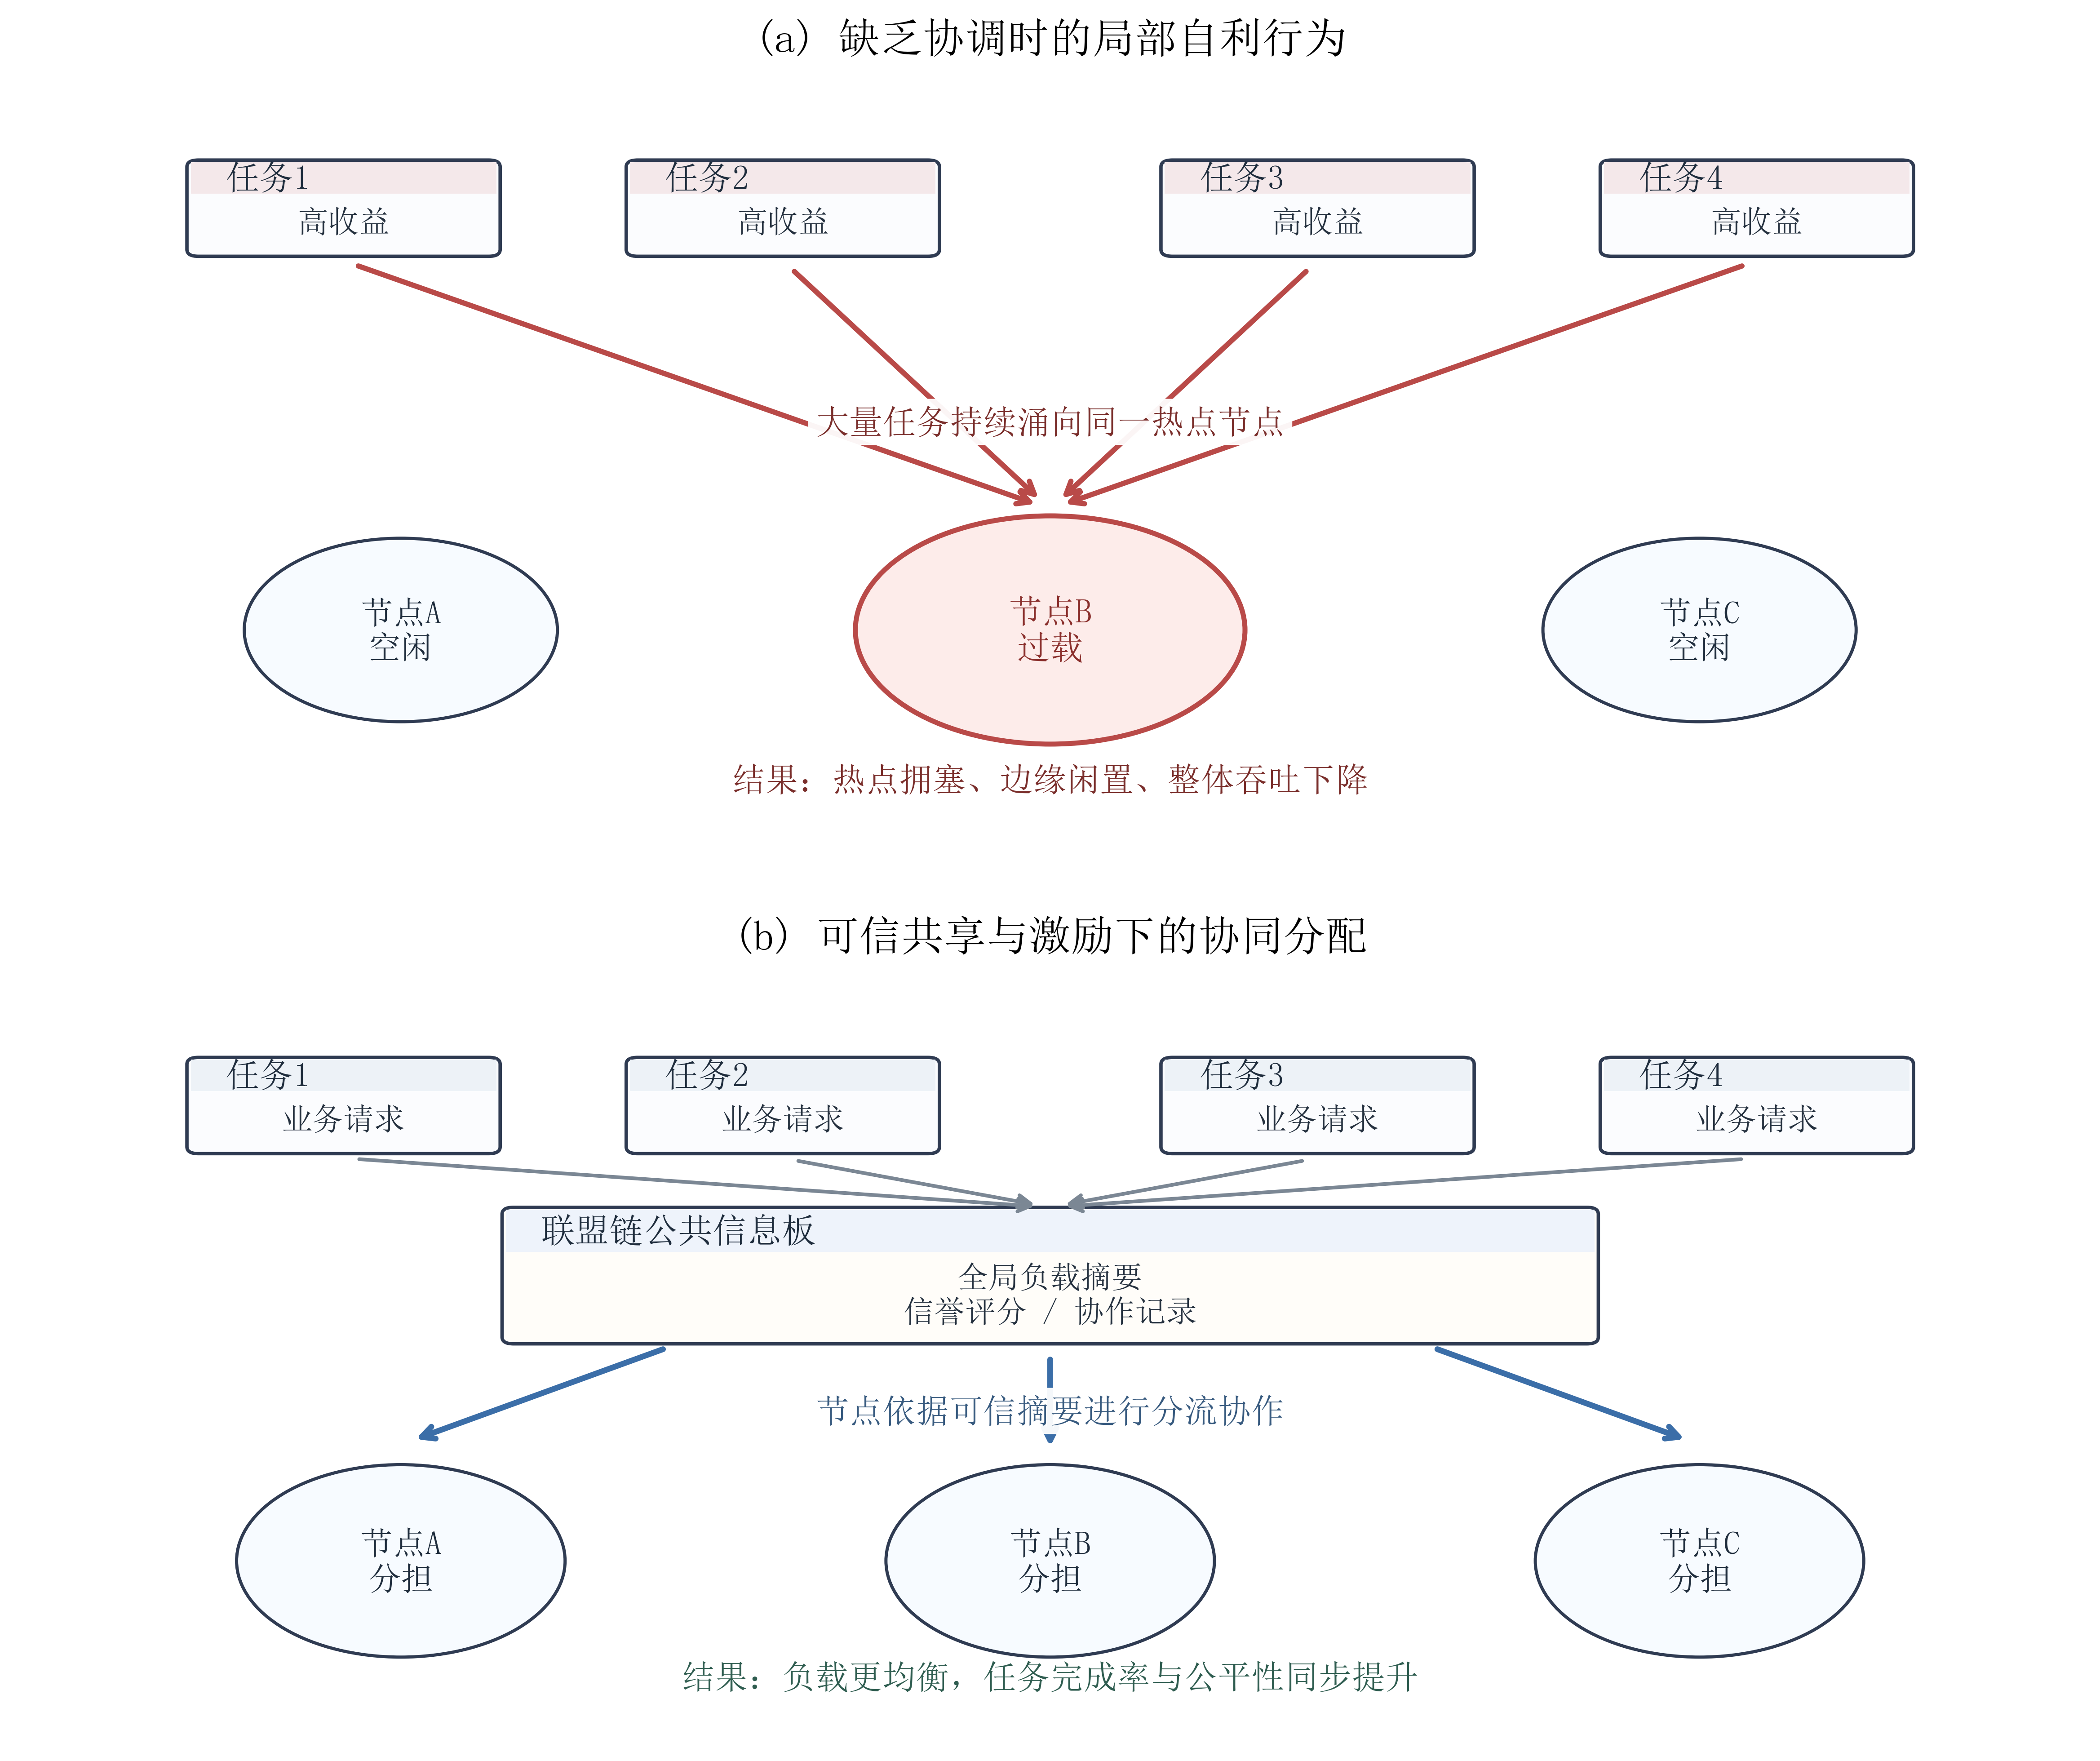
\includegraphics[width=0.94\textwidth]{images/3-new-1.png}
  \caption{天基协同资源分配中局部自利与全局协同差异示意}
  \label{fig:3_1}
\end{figure}

图~\ref{fig:3_1}从问题层面说明了本章研究对象的本质差异：在缺乏协调机制时，多个节点会同时追逐少量高收益任务，导致热点拥塞与资源浪费并存；而在可信共享与协同激励共同作用下，节点可形成更合理的任务分工、资源补偿与风险分摊关系，从而提升任务完成率、负载均衡度和长期运行稳定性。这一差异并不是简单的“调度策略优劣”问题，而是系统是否具备可靠公共上下文、是否存在长期激励约束、以及节点是否能够在动态环境中形成稳定协作关系的综合体现。

本章后续内容按照“系统框架—博弈建模—算法求解—实验验证”的逻辑展开。第 3.2 节首先给出系统参与者、联盟链公共信息板与协同流程的整体框架；第 3.3 节在此基础上建立多智能体马尔可夫博弈模型；第 3.4 节介绍区块链增强的 CTDE 多智能体强化学习求解方法；第 3.5 节通过多场景仿真实验验证所提方法在收敛性、负载均衡、任务完成率及抗自私行为方面的有效性；最后在第 3.6 节进行本章总结。

\section{系统框架概述}

为使后续建模与算法推导建立在清晰一致的系统图景之上，本节首先从系统组成、信息流转和协同目标三个方面，对本章所研究的天基协同资源分配框架进行概述。相较于直接进入公式化建模，这种“先框架、后抽象”的展开方式，更有助于说明各类状态、动作、奖励与联盟链要素在系统中的实际来源与功能定位。

\subsection{系统组成与角色划分}

本章考虑的天基计算网络由四类核心参与者共同构成：执行在轨任务的异构计算节点、负责状态记账与摘要广播的联盟链节点、承担本地调度与协同决策的智能体模块，以及在训练阶段负责全局价值评估的集中式训练协调器。四者既分工明确，又通过任务流、状态流与信誉流形成紧密耦合。

第一类参与者是\textbf{异构计算节点}。它们分布在不同轨道层和不同星座拓扑位置上，具备差异化的计算、存储、能量和通信能力，是在轨任务执行的直接承担者。对系统而言，每个节点既可能处理本地生成的任务，也可能接收其他节点卸载而来的任务，因此天然兼具“任务生产者”和“任务处理者”双重身份。

第二类参与者是\textbf{联盟链节点}。它们共同维护系统级公共摘要，包括节点负载、信誉评分、链路统计与历史行为记录等信息。联盟链并不替代实时调度器，而是充当“可信公共信息板”：一方面为各节点提供可审计、可验证、可追溯的系统级上下文；另一方面通过链上信誉累积和行为留痕机制，为后续的激励约束提供可信依据。

第三类参与者是\textbf{局部决策智能体}。每个计算节点内部均部署一个策略模块，依据本地私有状态与链上公共摘要联合决定任务是否本地执行、向哪个邻居卸载、投入多少本地资源以及是否接收外部任务。由于执行阶段无法依赖中心控制器，各节点必须具备在部分可观测条件下独立做出近实时决策的能力。

第四类参与者是\textbf{集中训练协调器}。它只在训练阶段存在，用于整合联合状态和联合动作，对多智能体策略进行价值评估与参数更新；在实际执行阶段，各节点仅保留各自的局部 Actor 网络，实现分散执行。这样的结构兼顾了训练阶段的信息利用效率与执行阶段的去中心化自治要求。

\begin{figure}[H]
  \centering
  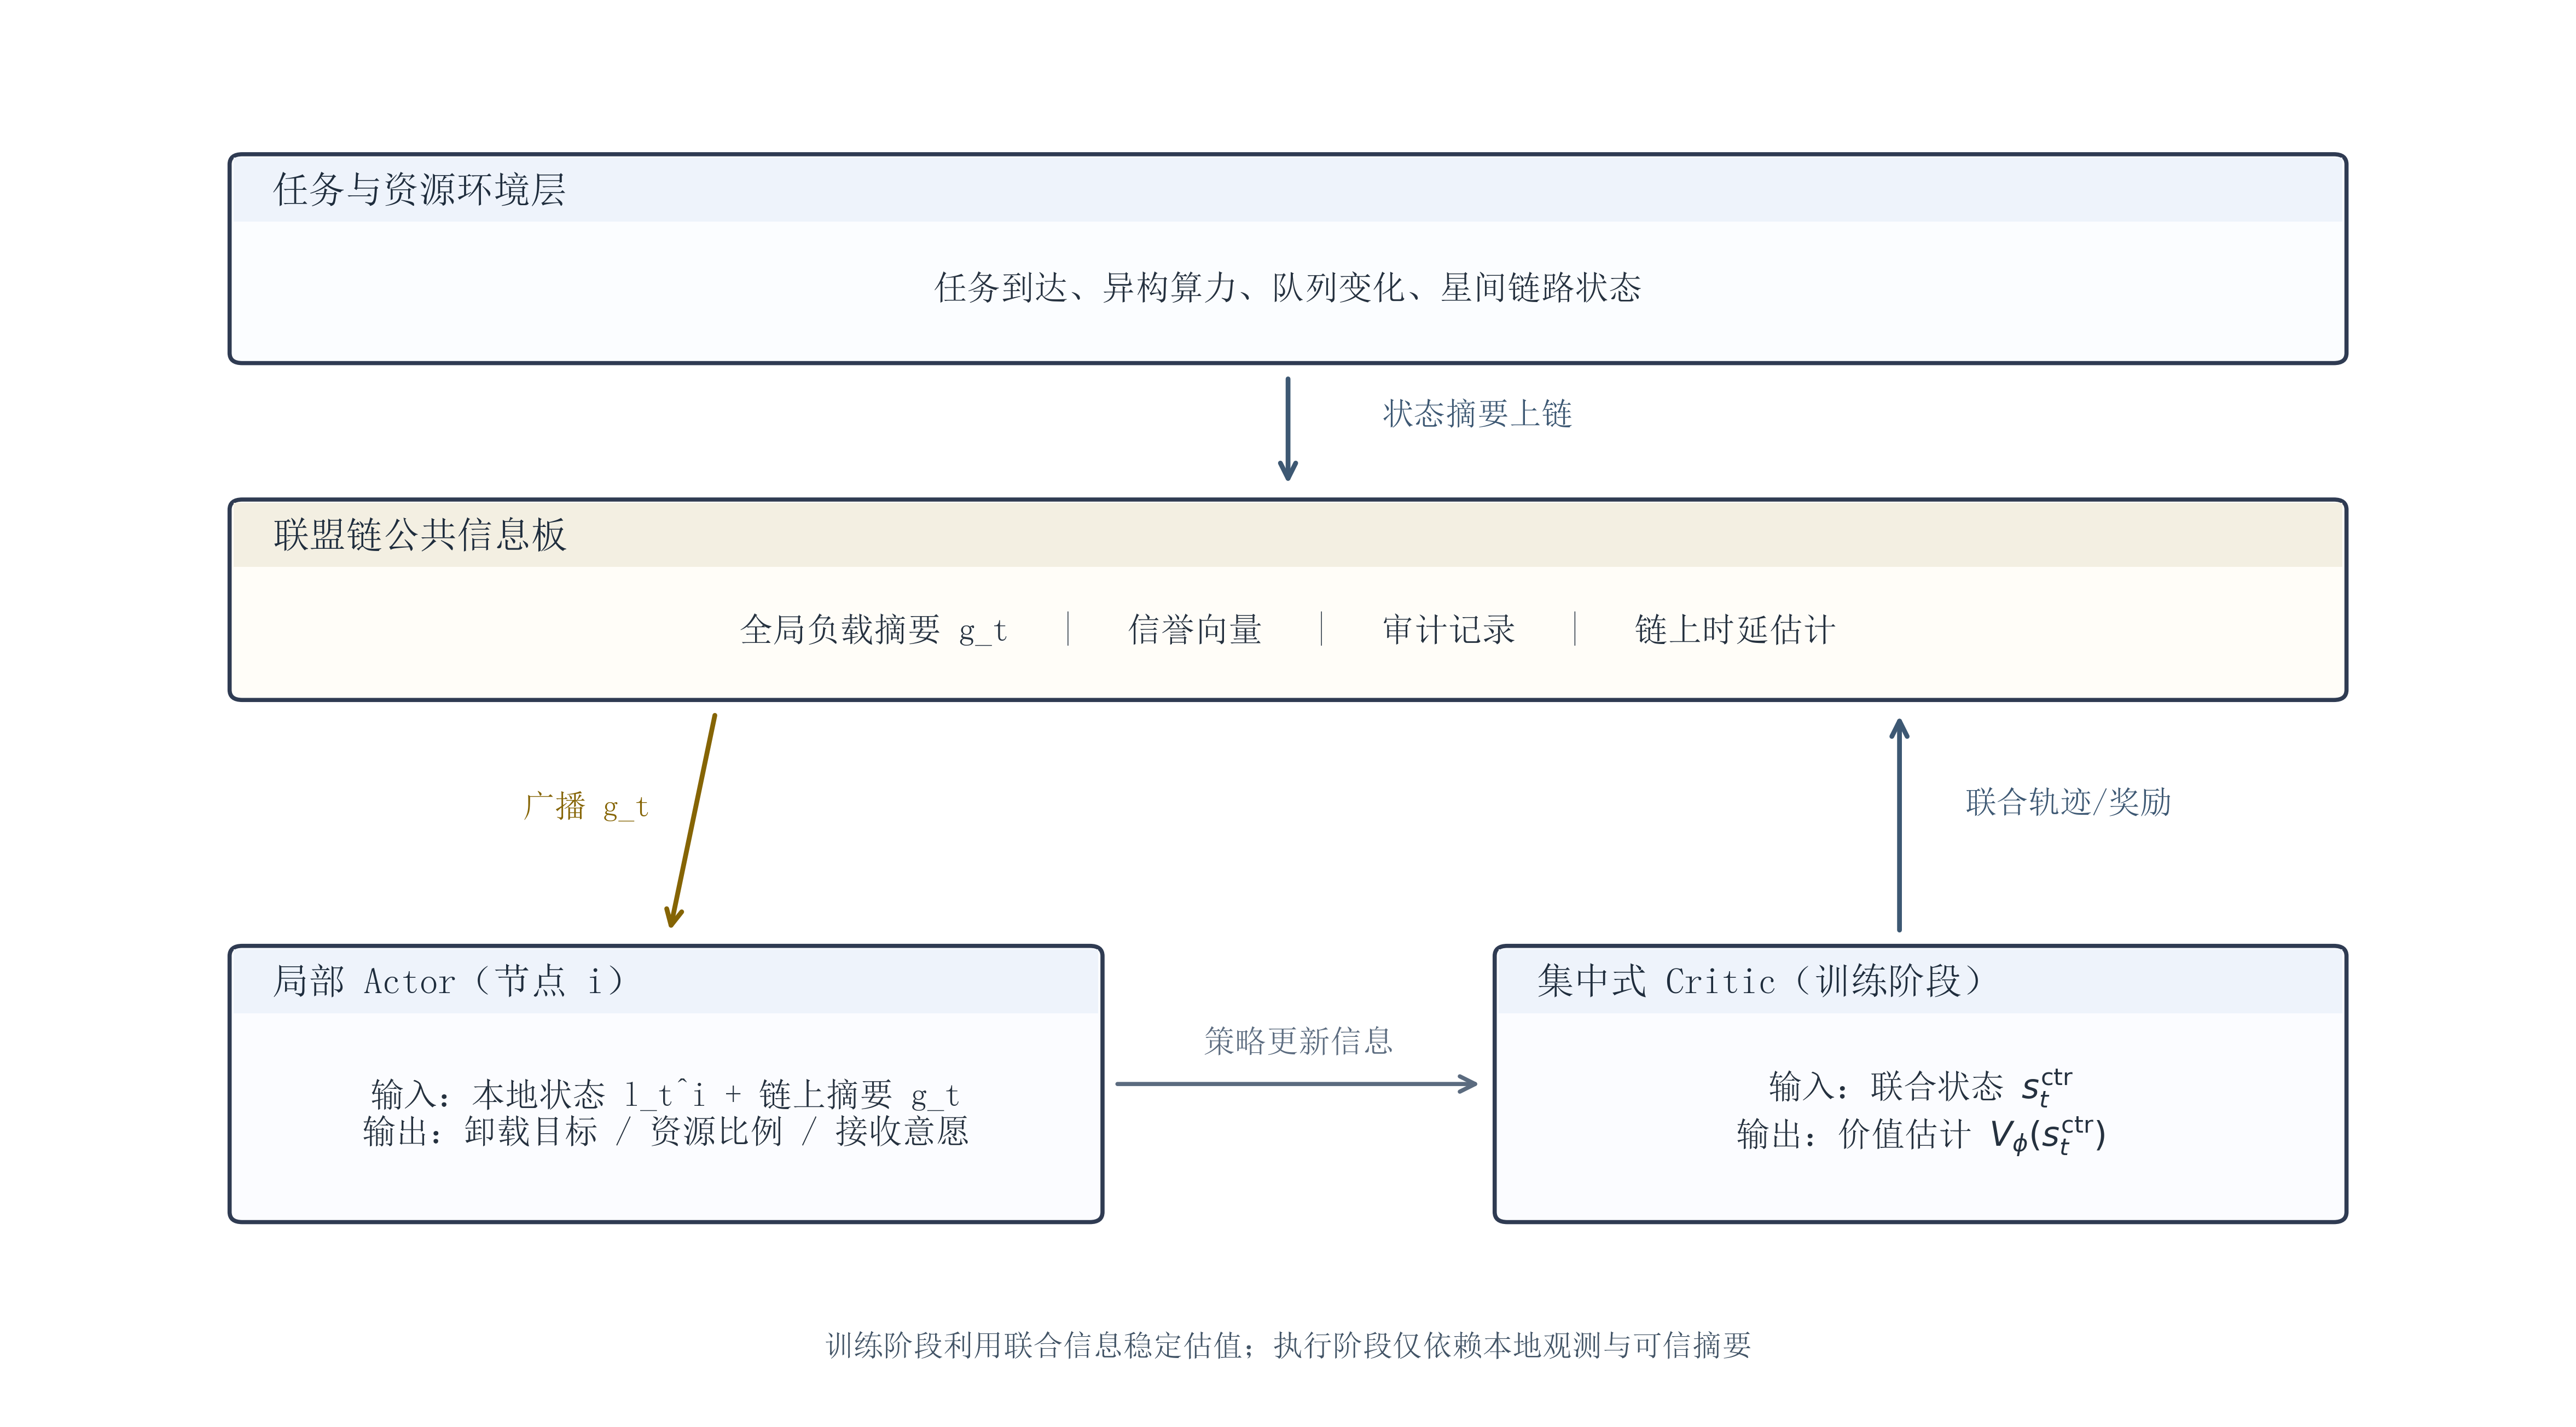
\includegraphics[width=0.94\textwidth]{images/3-new-4.png}
  \caption{第三章协同资源分配框架的层次结构与信息流}
  \label{fig:3_2}
\end{figure}

图~\ref{fig:3_2}给出了本章方法的整体层次结构。最上层为任务与资源环境层，描述任务持续到达、节点异构与链路变化等系统事实；中间层为联盟链公共信息板，负责对全局状态摘要、信誉演化与关键决策结果进行可信记录与广播；底层为各异构节点上的局部智能体，它们依据“本地观测 + 链上摘要”进行协同调度决策。训练阶段，集中式价值评估器通过汇聚联合信息更新策略参数；执行阶段，节点仅凭局部观测自主运行，从而形成“集中训练—分散执行”的闭环。

\subsection{联盟链公共信息板与协同流程}

在上述系统组成基础上，本章将协同资源分配过程组织为一个持续循环的闭环流程。不同于传统中心调度模式中“中心收集全局状态—中心下发动作”的单向控制链条，本章方法强调由联盟链维持公共上下文，由节点完成局部决策，再将执行反馈重新写回系统，从而实现可信共享与自主协同的统一。

具体而言，该协同流程可以概括为以下五个步骤。首先，\textbf{任务到达与本地感知}：当节点感知到新任务到达时，实时更新本地队列长度、CPU/内存利用率、剩余能量和当前工作负载等高频状态。其次，\textbf{链上摘要获取}：节点从联盟链读取全局平均负载、负载方差、链路统计、信誉评分和链上时延估计等低频但可信的公共摘要，用以补充局部感知中难以直接获得的系统级信息。再次，\textbf{局部协同决策}：策略网络基于“本地私有状态 + 链上公共摘要”输出卸载目标、资源分配比例和接收意愿等动作，并作用于当前节点。随后，\textbf{执行反馈与信誉更新}：动作执行后，系统会获得任务完成情况、平均时延、能耗、负载变化和协作质量等反馈，并据此更新节点信誉和系统负载摘要。最后，\textbf{链上记账与参数迭代}：联盟链将关键行为结果与信誉变化写入账本，在训练阶段进一步服务于全局价值评估和参数更新，在执行阶段则为下一轮协同决策提供新的可信上下文。

\begin{figure}[H]
  \centering
  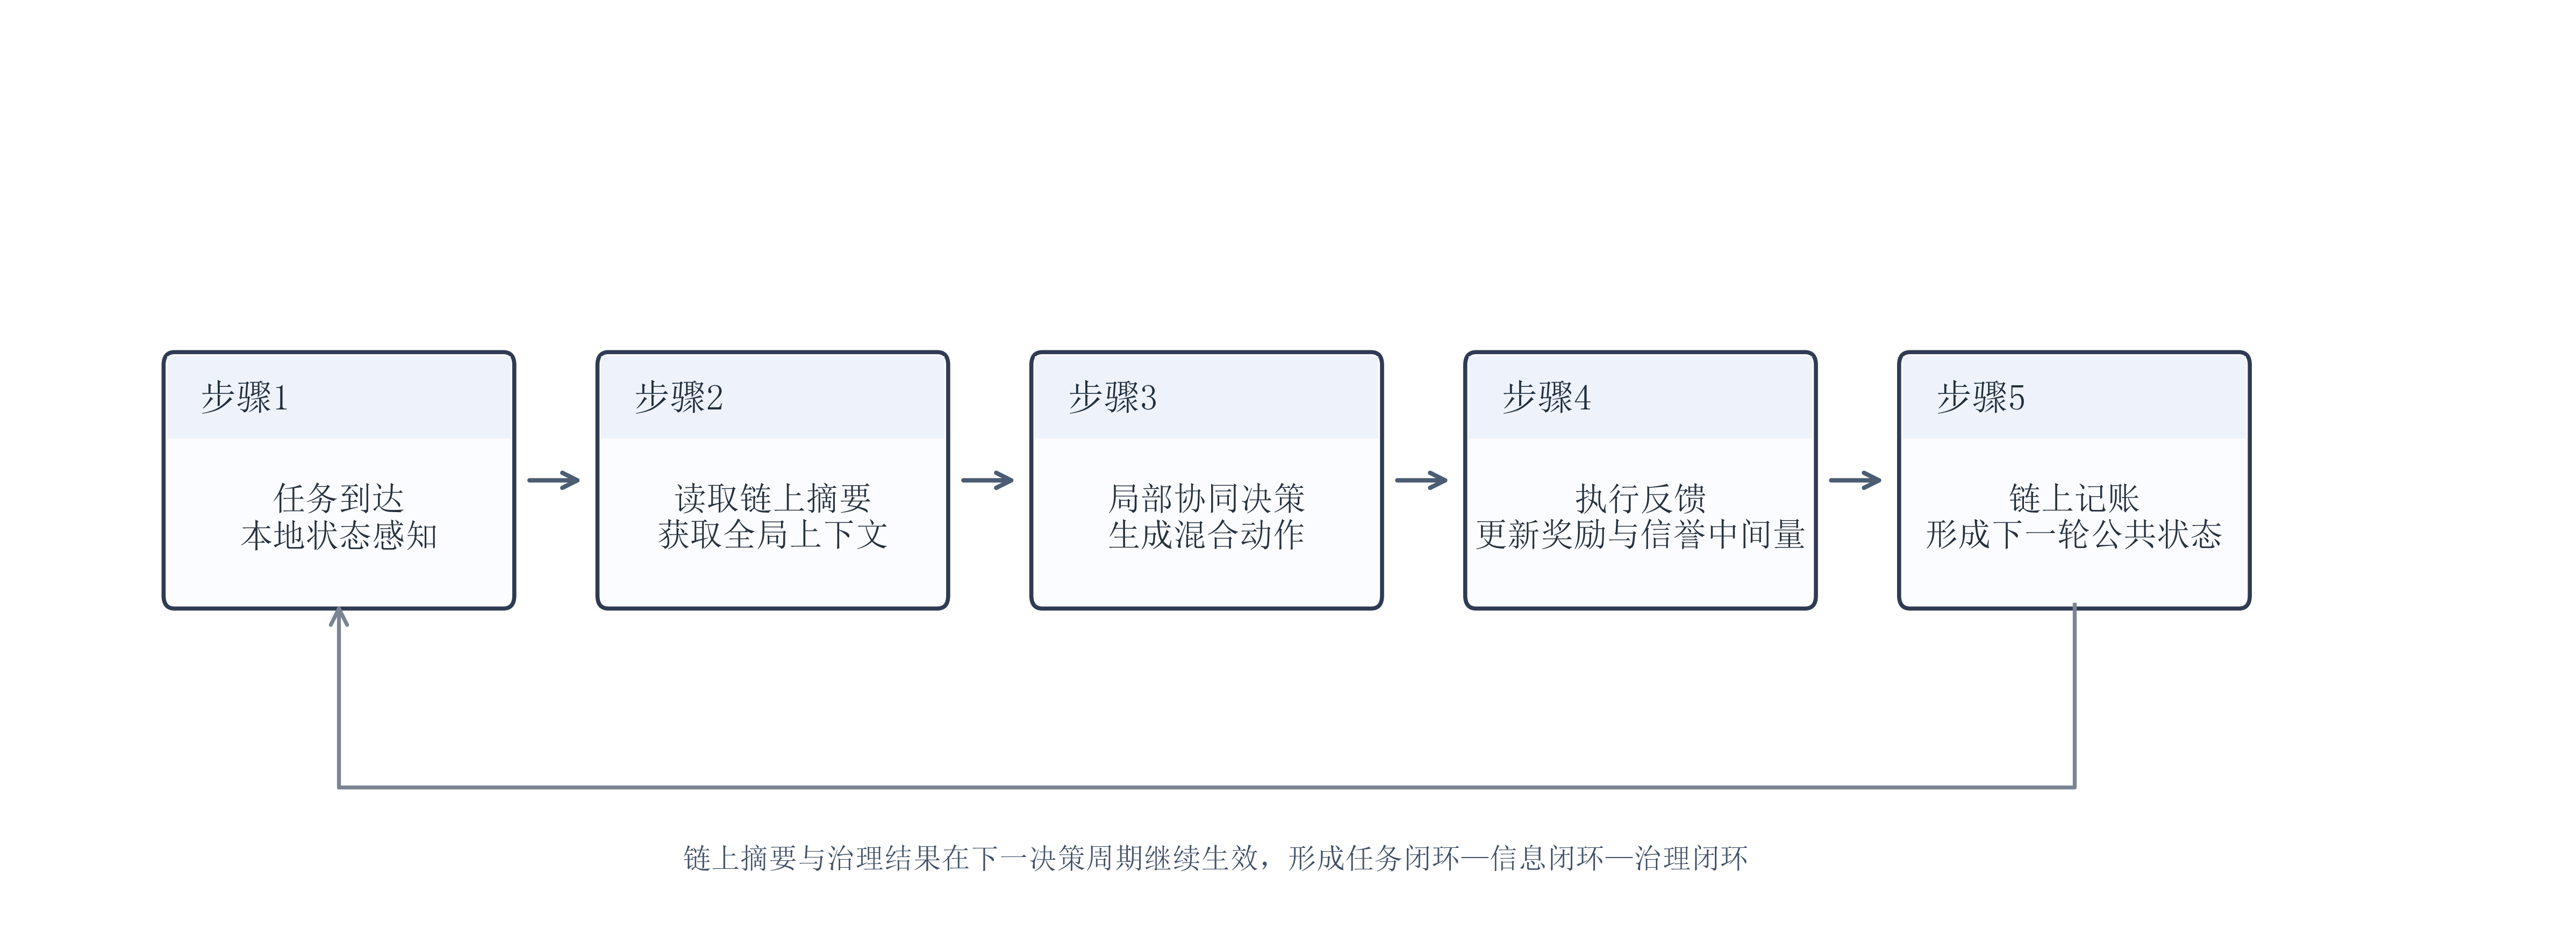
\includegraphics[width=0.92\textwidth]{images/3-new-5.png}
  \caption{基于联盟链公共信息板的任务—状态—信誉闭环协同流程}
  \label{fig:3_2_flow}
\end{figure}

图~\ref{fig:3_2_flow}强调了三个关键闭环：一是“任务到达—局部决策—执行反馈”的任务闭环，决定了系统的实时响应能力；二是“状态汇总—链上广播—节点读取”的信息闭环，决定了多节点之间能否在缺乏中心调度器的情况下获得统一的协同上下文；三是“协作行为—信誉变化—后续激励”的治理闭环，决定了系统能否对长期自利与机会主义偏离形成可持续约束。三者共同构成了本章后续博弈建模与强化学习求解的系统基础。

\subsection{建模目标与协同难点}

在上述框架下，本章关注的核心问题可以概括为：当任务持续动态到达系统后，多个异构节点如何在不依赖中心调度器的条件下，联合决定任务由谁处理、何时处理、是否接纳外部卸载以及投入多少本地资源，使系统整体在任务完成率、平均时延、能耗开销、负载均衡和协同可信性之间取得更优平衡。换言之，本章研究的不是静态任务指派问题，而是一个随任务流、资源状态、链路关系和信誉轨迹不断演化的多主体序贯决策问题。

这一问题之所以困难，主要来自四类耦合难点。其一是\textbf{资源异构与收益非一致性}：相同任务在不同节点上的执行代价、完成收益和机会成本并不相同，局部最优动作往往会诱导全局失衡。其二是\textbf{任务到达与链路状态的时变性}：任务负载具有突发与长尾特征，链路可用性则随轨道位置和拥塞条件动态变化，使得调度策略必须具备在线适应能力。其三是\textbf{可信共享信息的时效性约束}：联盟链提供了可验证的系统级上下文，但链上信息同步本身存在时延，节点决策必须同时考虑“信息可信”与“信息陈旧”两种因素。其四是\textbf{自利行为与长期治理问题}：节点会根据局部收益结构动态调整行为，若缺少信誉约束和公共审计机制，系统容易重新滑向任务热点聚集与协作退化。

因此，从方法论角度看，后续建模必须同时满足三点要求：一是能够刻画多节点之间“策略—环境”双向耦合的动态交互；二是能够把联盟链提供的可信公共摘要纳入状态建模与激励设计；三是能够在训练阶段充分利用联合信息、在执行阶段保持局部自治。基于这一认识，下一节将进一步把上述系统框架形式化为多智能体马尔可夫博弈模型，并为后续的区块链增强 CTDE 求解方法奠定数学基础。

\section{基于多智能体马尔可夫博弈的协同资源分配建模}

第 3.2 节已经从系统组成、联盟链公共信息板与任务—状态—信誉闭环流程三个方面，建立了本章方法的整体框架，并指出该问题的核心困难不仅在于组合优化层面的计算压力，更在于多个理性决策主体在信息不对称、利益冲突和长期收益耦合条件下的策略交互。由此可见，若仅依赖集中式全局优化方法，虽然理论上能够给出某种最优解，但其对全局信息实时可获取性的要求与天基网络固有的去中心化约束形成根本矛盾；若采用单智能体马尔可夫决策过程（MDP），又会将其他节点的策略变化等价地视为环境扰动，从而无法刻画多节点之间“策略—环境”双向耦合的本质。因此，本文选择以多智能体马尔可夫博弈（Multi-Agent Markov Game, MAMG）作为系统层协同资源分配的统一建模框架，并在此基础上进一步引入区块链公共信息板与信誉驱动机制，使抽象博弈模型能够在去中心化场景中落地执行。

\subsection{建模动机与博弈形式化}

在将协同资源分配问题映射到数学框架之前，有必要首先说明为何采用马尔可夫博弈而非标准形式博弈或重复博弈。标准形式博弈仅适用于一次性策略选择，无法表达资源状态随时间演化的序贯特征；重复博弈虽考虑多轮交互，但默认每一轮都在相同阶段博弈上重复进行，并不显式刻画系统状态随联合动作变化而转移的机制。然而，在天基计算网络中，任何一次任务卸载决策都会改变后续时刻的队列长度、资源占用率、链路可用性与信誉演化轨迹，即当前动作会通过状态转移持续影响未来收益。因此，该问题本质上是一个多主体、序贯式、状态相关的动态博弈问题。

基于上述认识，本文将 $N$ 个异构边缘计算节点的协同调度问题形式化为如下七元组：
\begin{equation}
  \mathcal{G}=\langle N,\,S,\,\{A^i\},\,P,\,\{R^i\},\,\gamma,\,\{O^i\}\rangle,
  \label{eq:margov_game}
\end{equation}
其中，$N$ 表示智能体集合，$S$ 表示全局状态空间，$A^i$ 表示节点 $i$ 的动作空间，$P$ 表示联合状态转移函数，$R^i$ 表示节点 $i$ 的即时奖励函数，$\gamma\in[0,1)$ 为折扣因子，$O^i$ 表示局部观测函数。

需要特别指出的是，天基计算网络并不满足完全信息博弈假设。受限于星间链路的间歇连通性、有限带宽和状态同步代价，任何单个节点都不可能实时获得所有远端节点的完整原始状态。因此，本文将该问题进一步建模为部分可观测的多智能体马尔可夫博弈。对节点 $i$ 而言，其在时刻 $t$ 的观测表示为
\begin{equation}
  o_t^i = O^i(s_t),
  \label{eq:obs_func}
\end{equation}
其中 $s_t$ 表示时刻 $t$ 的全局状态，$o_t^i$ 属于节点 $i$ 的局部观测空间 $\Omega^i$。相应地，每个节点维护一个随机化策略 $\pi^i:\Omega^i\to \Delta(A^i)$，并以最大化期望累积折扣回报为目标：
\begin{equation}
  J^i(\pi^i,\pi^{-i})=\mathbb{E}\!\left[\sum_t\gamma^t R^i\!\left(s_t,a_t^i,a_t^{-i},s_{t+1}\right)\mid \pi^i,\pi^{-i}\right],
  \label{eq:return}
\end{equation}
这里 $\pi^{-i}$ 表示除节点 $i$ 之外其余所有节点的联合策略。上述目标函数表明，节点 $i$ 的收益不仅取决于自身策略，还显式依赖于其他节点的策略组合，这也是单智能体强化学习框架难以直接适配该问题的根本原因。

\begin{figure}[H]
  \centering
  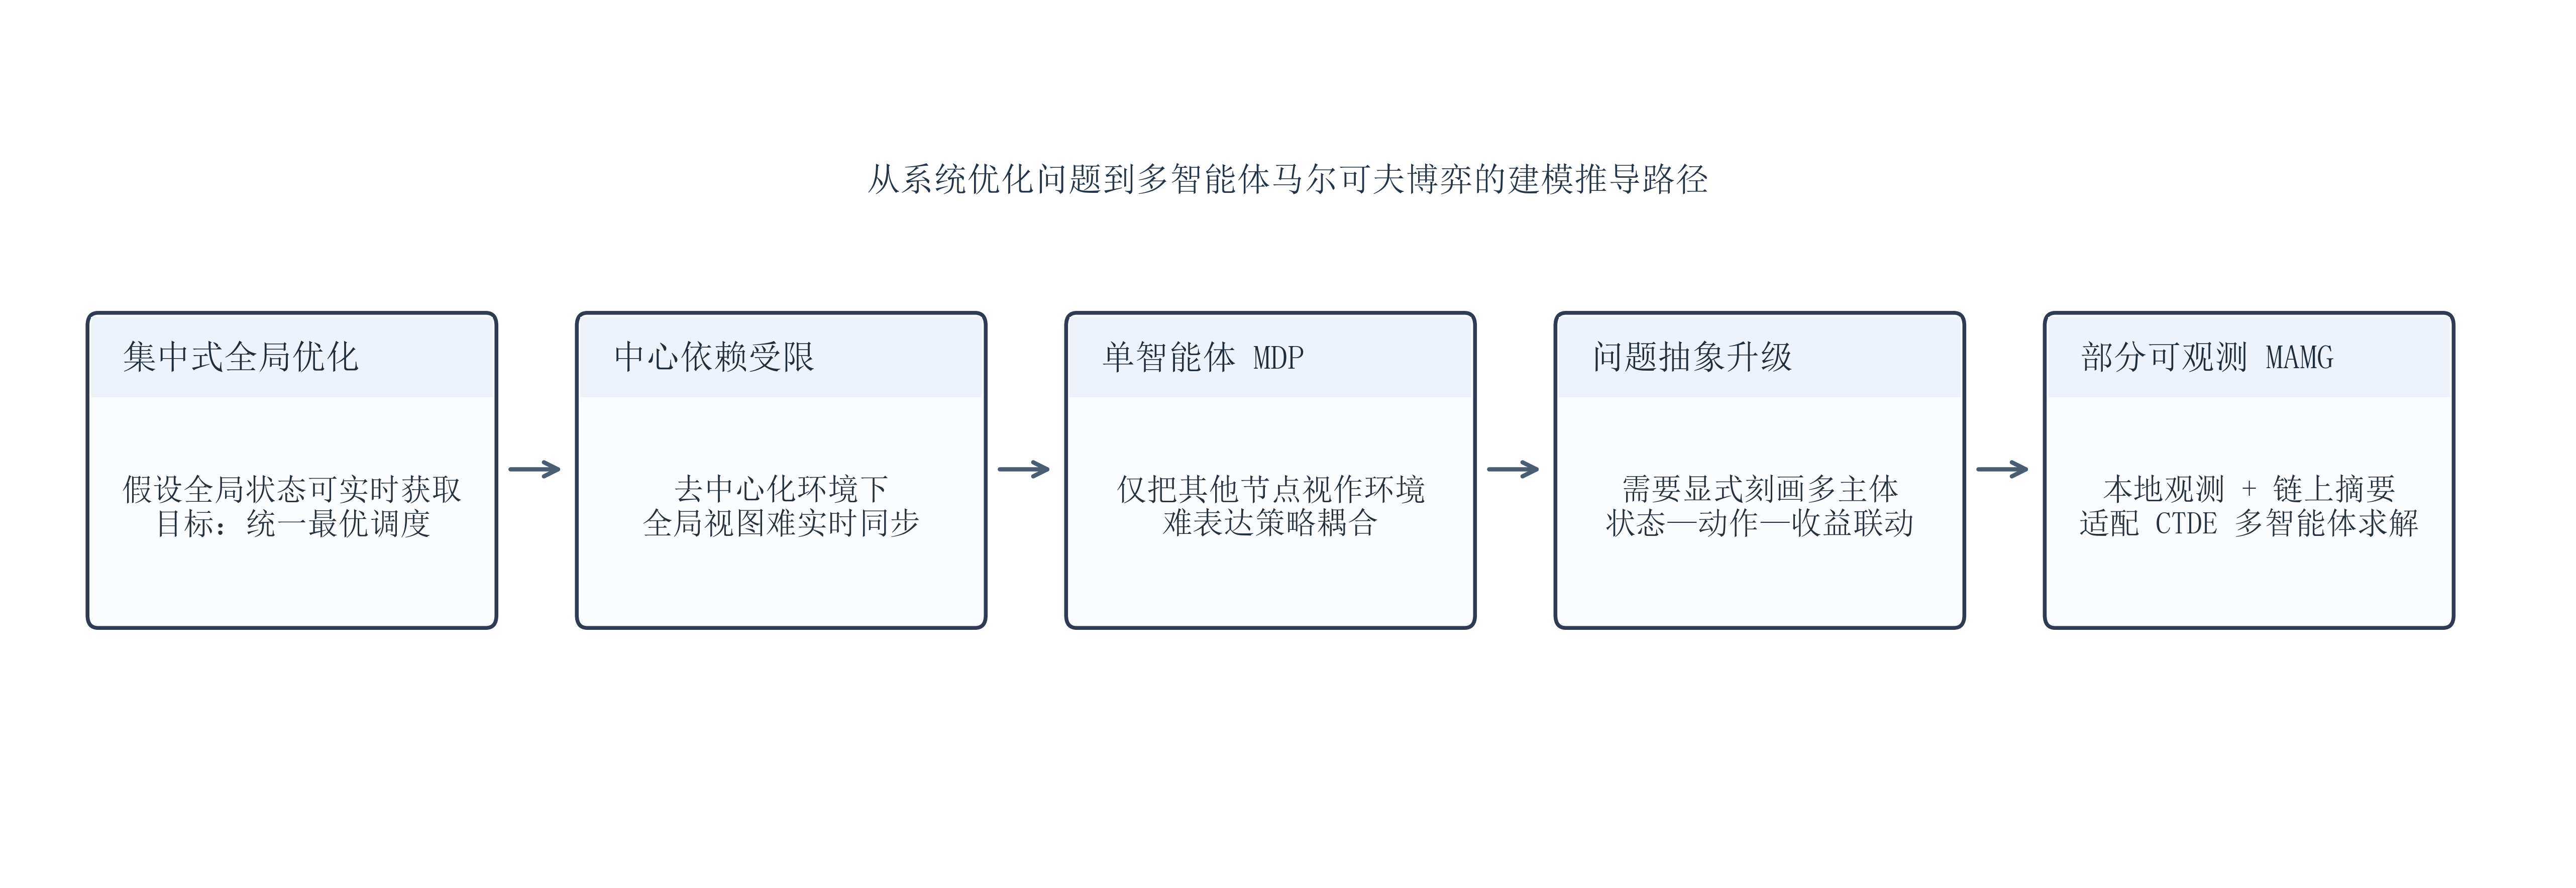
\includegraphics[width=0.94\textwidth]{images/3-new-3.png}
  \caption{从系统优化问题到多智能体马尔可夫博弈的建模推导路径}
  \label{fig:3_3}
\end{figure}

\subsection{状态、动作与奖励机制设计}

在明确了博弈形式之后，接下来需要回答一个更具体的问题：节点究竟基于什么信息决策、能够采取哪些行动，以及系统希望通过何种奖励塑形引导节点从个体理性走向集体理性。对此，本文分别从状态空间、动作空间和奖励机制三个层面进行设计。

首先，在状态空间设计上，需要在“信息充分性”和“维度可控性”之间取得平衡。若观测过于贫乏，节点将因缺乏必要上下文而难以形成有效策略；但若直接纳入过多原始任务级信息，又会导致状态维度膨胀，增加训练难度与通信开销。为此，本文将节点 $i$ 在时刻 $t$ 的观测结构化为“本地私有状态 + 链上公共摘要”两部分：
\begin{equation}
  o_t^i = \left(l_t^i,\,g_t\right),
  \label{eq:obs_split}
\end{equation}
其中，本地私有状态 $l_t^i$ 由节点自行采集，表示为
\begin{equation}
  l_t^i = \left(Q_t^i,\,\rho_{\mathrm{cpu}}^i(t),\,\rho_{\mathrm{mem}}^i(t),\,E_t^i,\,h_i,\,w_t^i\right),
  \label{eq:local_state}
\end{equation}
这里 $Q_t^i$ 为本地队列长度，$\rho_{\mathrm{cpu}}^i(t)$ 和 $\rho_{\mathrm{mem}}^i(t)$ 分别为 CPU 与内存利用率，$E_t^i$ 表示剩余能量预算或累计能耗，$h_i$ 为节点静态硬件特征向量，$w_t^i$ 概括当前工作负载信息。另一方面，链上公共摘要 $g_t$ 由联盟链周期性聚合并广播，表示为
\begin{equation}
  g_t = \left(\bar{L}_t,\,\sigma_L^2(t),\,D_t^{\mathrm{task}},\,R_t^{\mathrm{rep}},\,\hat{D}_{\mathrm{chain}}(t),\,T_t^{\mathrm{stat}}\right),
  \label{eq:global_summary}
\end{equation}
其中 $\bar{L}_t$ 表示全局平均负载，$\sigma_L^2(t)$ 表示负载方差，$D_t^{\mathrm{task}}$ 为任务分布摘要，$R_t^{\mathrm{rep}}$ 为信誉评分向量，$\hat{D}_{\mathrm{chain}}(t)$ 为链上同步延迟估计，$T_t^{\mathrm{stat}}$ 为吞吐量统计摘要。

\begin{table}[H]
\centering
\caption{链上公共摘要分量说明}
\label{tab:summary}
\begin{tabularx}{\textwidth}{C{2.3cm}C{2.2cm}Y}
\toprule
分量 & 名称 & 说明 \\
\midrule
$\bar{L}_t$ & 全局平均负载 & 所有节点队列长度的加权均值，反映系统整体繁忙程度 \\
$\sigma_L^2(t)$ & 负载方差 & 各节点负载的离散程度，衡量系统均衡性 \\
$D_t^{\mathrm{task}}$ & 任务分布摘要 & 各类型任务在网络中的分布统计，用于感知业务结构变化 \\
$R_t^{\mathrm{rep}}$ & 信誉评分向量 & 各节点的链上信誉评分，反映历史行为质量 \\
$\hat{D}_{\mathrm{chain}}(t)$ & 链上延迟估计 & 共识与数据同步的当前延迟估计值，用于补偿信息滞后 \\
$T_t^{\mathrm{stat}}$ & 吞吐量统计 & 近期各节点及系统整体吞吐量的滑动统计，用于辅助协同判断 \\
\bottomrule
\end{tabularx}
\end{table}

值得注意的是，$R_t^{\mathrm{rep}}$ 为信誉约束提供了可信输入，而 $\hat{D}_{\mathrm{chain}}(t)$ 的显式纳入使节点能够感知当前信息时效性，并在策略中对链上同步滞后进行自适应补偿。

其次，在动作空间设计上，原始调度决策天然包含离散与连续两类分量：节点既要决定任务是本地执行还是卸载给哪个邻居，也要决定本地资源分配比例以及是否愿意接收外部任务。若直接将“逐任务优先级向量”作为动作输出，其维度会随队列长度变化，不利于神经网络策略表示与训练稳定性。因此，本文采用固定维混合动作表示：
\begin{equation}
  a_t^i = \left(a_{\mathrm{off},t}^i,\,a_{\mathrm{res},t}^i,\,a_{\mathrm{acc},t}^i\right),
  \label{eq:hybrid_action}
\end{equation}
其中 $a_{\mathrm{off},t}^i$ 表示卸载目标选择，$a_{\mathrm{res},t}^i\in[0,1]$ 表示本地资源分配比例，$a_{\mathrm{acc},t}^i\in[0,1]$ 表示接收外部任务的意愿系数。对于本地队列内部的细粒度排序，本文不再将其直接作为策略网络输出，而是通过一个基于任务时延约束、计算量和信誉补偿的规则化排序器在节点本地生成。这样既能保持 Actor 输出维度固定，又实现了“高层学协同、低层做排序”的结构化解耦。

最后，在奖励机制设计上，若仅以本地吞吐或完成收益作为奖励，节点策略将自然倾向于争抢高价值任务并规避低收益协作，从而重演前文所分析的公地悲剧。为此，本文构建融合效率、公平与可信性的三维混合奖励函数：
\begin{equation}
  r_t^i = w_q r_{q,t}^i + w_f r_{f,t}^i + w_c r_{c,t}^i,
  \label{eq:hybrid_reward}
\end{equation}
其中 $w_q,w_f,w_c\ge 0$ 且 $w_q+w_f+w_c=1$。效率项用于刻画节点自身任务处理质量，可写为
\begin{equation}
  r_{q,t}^i = \alpha_1\mathrm{Succ}_t^i - \alpha_2\mathrm{Delay}_t^i - \alpha_3\mathrm{Energy}_t^i,
  \label{eq:rq}
\end{equation}
其中 $\mathrm{Succ}_t^i$ 为成功完成任务数，$\mathrm{Delay}_t^i$ 为平均完成时延，$\mathrm{Energy}_t^i$ 为单位时间能耗。公平项用于引导系统整体负载均衡，本文采用基于 Jain 公平指数的全局度量\cite{ref6}：
\begin{equation}
  J_t = \frac{\left(\sum_i x_i(t)\right)^2}{N\sum_i x_i^2(t)},
  \label{eq:jain}
\end{equation}
其中 $x_i(t)$ 表示节点 $i$ 的有效服务率或负载承担量，进而定义
\begin{equation}
  r_{f,t}^i = J_t - \beta\,\max\left\{0,\,\rho_i(t)-\rho_{\mathrm{th}}\right\}.
  \label{eq:rf}
\end{equation}
可信性项则将节点历史行为纳入激励闭环：
\begin{equation}
  r_{c,t}^i = \gamma_1 \Delta \mathrm{Rep}_i(t) - \gamma_2 \delta_i(t),
  \label{eq:rc}
\end{equation}
其中 $\Delta \mathrm{Rep}_i(t)$ 表示信誉增量，$\delta_i(t)$ 表示负载偏差度。诚实上报与积极协同的节点将获得正向激励，虚报状态和拒绝协作的节点则受到惩罚。

\begin{table}[H]
\centering
\caption{奖励权重与作用说明}
\label{tab:reward_weight}
\begin{tabularx}{\textwidth}{C{1.8cm}C{2.2cm}Y C{1.5cm}}
\toprule
权重 & 对应项 & 核心作用 & 默认值 \\
\midrule
$w_q$ & 效率项 $r_q$ & 保证任务完成率、时延与能耗三者的局部效率优化 & 0.5 \\
$w_f$ & 公平项 $r_f$ & 抑制热点拥塞，提升系统负载均衡与长期稳定性 & 0.3 \\
$w_c$ & 可信项 $r_c$ & 将信誉增量与负载偏差反馈到策略更新中，约束欺骗行为 & 0.2 \\
\bottomrule
\end{tabularx}
\end{table}

\subsection{约束条件与性质分析}

作为一个面向真实天基计算网络的协同调度模型，上述博弈并非在抽象无限制环境中运行，而必须满足物理资源约束与通信可行性约束。对任意节点 $i$ 而言，首先有基本的本地资源约束：
\begin{equation}
  0 \le a_{\mathrm{res},t}^i \le 1,
  \label{eq:res_ratio}
\end{equation}
\begin{equation}
  C_i^{\mathrm{used}}(t)\le C_i^{\max},\quad
  B_i^{\mathrm{used}}(t)\le B_i^{\max},\quad
  E_i^{\mathrm{used}}(t)\le E_i^{\mathrm{cap}},
  \label{eq:resource_const}
\end{equation}
其中 $C_i^{\mathrm{used}}(t)$、$B_i^{\mathrm{used}}(t)$、$E_i^{\mathrm{used}}(t)$ 分别表示时刻 $t$ 的计算资源占用、带宽占用和能量消耗。当节点选择执行卸载动作时，相应任务的数据传输量还必须满足链路带宽预算和可见窗口约束。本文在环境层通过动作可行性检查与不可行动作惩罚共同保证策略学习始终发生在物理可行域内。

在满足上述约束的前提下，还需要讨论模型在理论上的可解释性。需要说明的是，原始问题同时包含离散卸载选择与连续资源比例控制，严格意义上的全局均衡求解较为困难。因此，本文并不试图对原始离散—连续混合博弈给出过强的解析结论，而是在混合策略和连续松弛意义下给出两个性质说明。

\textbf{定理 3.1（连续松弛下的均衡存在性）} 在各智能体采用混合策略、奖励函数对联合策略连续，且连续动作空间为非空紧凸集的条件下，所构造的松弛博弈至少存在一个混合策略纳什均衡\cite{ref7}。

该结论可由 Glicksberg 不动点定理得到。需要强调的是，这里讨论的是连续松弛后的策略博弈，其意义在于说明本文设计的奖励结构与策略表示不会破坏均衡存在性，而非声称原始混合动作博弈在所有条件下都可直接解析求解。

\textbf{定理 3.2（局部稳定性说明）} 若在某一局部邻域内，联合策略更新可近似表示为对某个光滑潜在函数的上升过程，且学习率足够小，则策略迭代在该邻域内具有局部稳定性。

该性质为后续采用 MAPPO 求解提供理论直觉：通过将公平项与信誉项嵌入奖励函数，不同节点的局部优化方向在一定程度上得到对齐，从而减弱了纯竞争博弈中常见的剧烈震荡现象。这里给出的并非严格的全局收敛证明，而是对训练稳定性来源的性质解释。


在上述状态、动作、奖励与约束设计的基础上，本节已经回答了‘系统希望节点依据什么信息决策、能够采取哪些行动、以及为何通过混合奖励塑形来抑制公地悲剧’这三个核心问题。换言之，第 3.3 节完成的是**问题求解对象的数学抽象**：它把第 3.2 节中的系统角色、链上公共摘要与信誉治理机制统一映射为一个部分可观测、多主体、序贯式的动态博弈模型，并说明了该模型在物理可行域内的基本性质。

但仅有建模仍不足以直接落地到天基网络的在线协同决策。原因在于：第一，联合状态与联合动作维度随节点数量增长而迅速膨胀；第二，Actor 在执行阶段只能访问局部观测与链上摘要，不能依赖训练期的全局信息；第三，链上公共信息板虽然提供了可信共享与审计能力，但其时延、更新周期和信誉回写机制必须被纳入具体的学习与执行流程，才能真正转化为策略性能增益。因此，下一节将从“如何求解”而非“如何建模”的角度出发，把上述马尔可夫博弈进一步映射为区块链增强的集中训练—分散执行多智能体强化学习框架，并说明策略参数更新、链上共享、信誉反馈和在线部署之间的耦合关系。

\section{区块链增强的 CTDE-MAPPO 协同算法设计}

上一节从系统约束、局部观测、混合动作和三维奖励塑形四个方面完成了协同资源分配问题的博弈建模，但这仍停留在“优化目标与交互结构已被定义”的层面。要使该模型真正用于天基网络在线运行，还需要进一步解决两个实现性问题：其一，在多节点联合策略持续变化的条件下，如何缓解多智能体学习中的环境非平稳性；其二，链上公共摘要与信誉反馈如何嵌入参数更新与在线执行过程，而不是停留在建模假设中。基于此，本节从求解层面对第 3.3 节的博弈模型进行算法化实现，构建区块链增强的集中训练—分散执行多智能体强化学习框架 BC-CTDE-MAPPO。

该框架的核心思想是：在训练阶段，利用联合状态近似表示、链上公共摘要与全局回报信号构造集中式 Critic，以降低多智能体环境中的策略漂移；在执行阶段，各节点仅保留本地私有状态与联盟链广播的可信摘要作为决策输入，维持去中心化自治；同时，链上公共信息板不仅提供系统级上下文，还承担信誉更新、行为审计与异常约束的反馈通道，使“可信共享—策略优化—治理回写”三者形成统一闭环。按照这一思路，本节依次介绍算法总体框架、混合动作策略与参数更新机制、区块链共享与信誉反馈机制，以及训练—执行一体化流程。

\subsection{算法总体框架}

设节点 $i$ 的 Actor 参数为 $\theta_i$，共享 Critic 参数为 $\phi$。在时刻 $t$，节点首先从本地环境与联盟链中读取观测 $o_t^i=(l_t^i,g_t)$，然后按照当前策略采样混合动作 $a_t^i=(a_{\mathrm{off},t}^i,a_{\mathrm{res},t}^i,a_{\mathrm{acc},t}^i)$。环境执行联合动作 $a_t=(a_t^1,\ldots,a_t^N)$ 后，更新任务队列、链路状态、能耗状态与信誉中间量，并将新的链上摘要写入公共信息板。随后，系统依据式~(\ref{eq:hybrid_reward}) 定义的三维奖励函数计算各节点即时回报 $r_t^i$，并将交互轨迹存入 rollout 缓冲区。一个 rollout 周期结束后，集中训练模块基于联合轨迹估计优势函数并更新 Actor/Critic 参数。

其中，集中式 Critic 的输入为全局状态近似表示
\begin{equation}
  s_t^{\mathrm{ctr}}=(l_t^1,\ldots,l_t^N,g_t),
  \label{eq:central_state}
\end{equation}
输出价值估计 $V_\phi(s_t^{\mathrm{ctr}})$。考虑到天基网络拓扑随时间动态变化，本文在状态编码阶段引入图结构聚合器，用于对邻接节点状态和链路关系进行表征学习。这样，一方面能够避免简单拼接带来的维度膨胀，另一方面也使价值网络具备对拓扑动态变化的敏感性。

\begin{figure}[H]
  \centering
  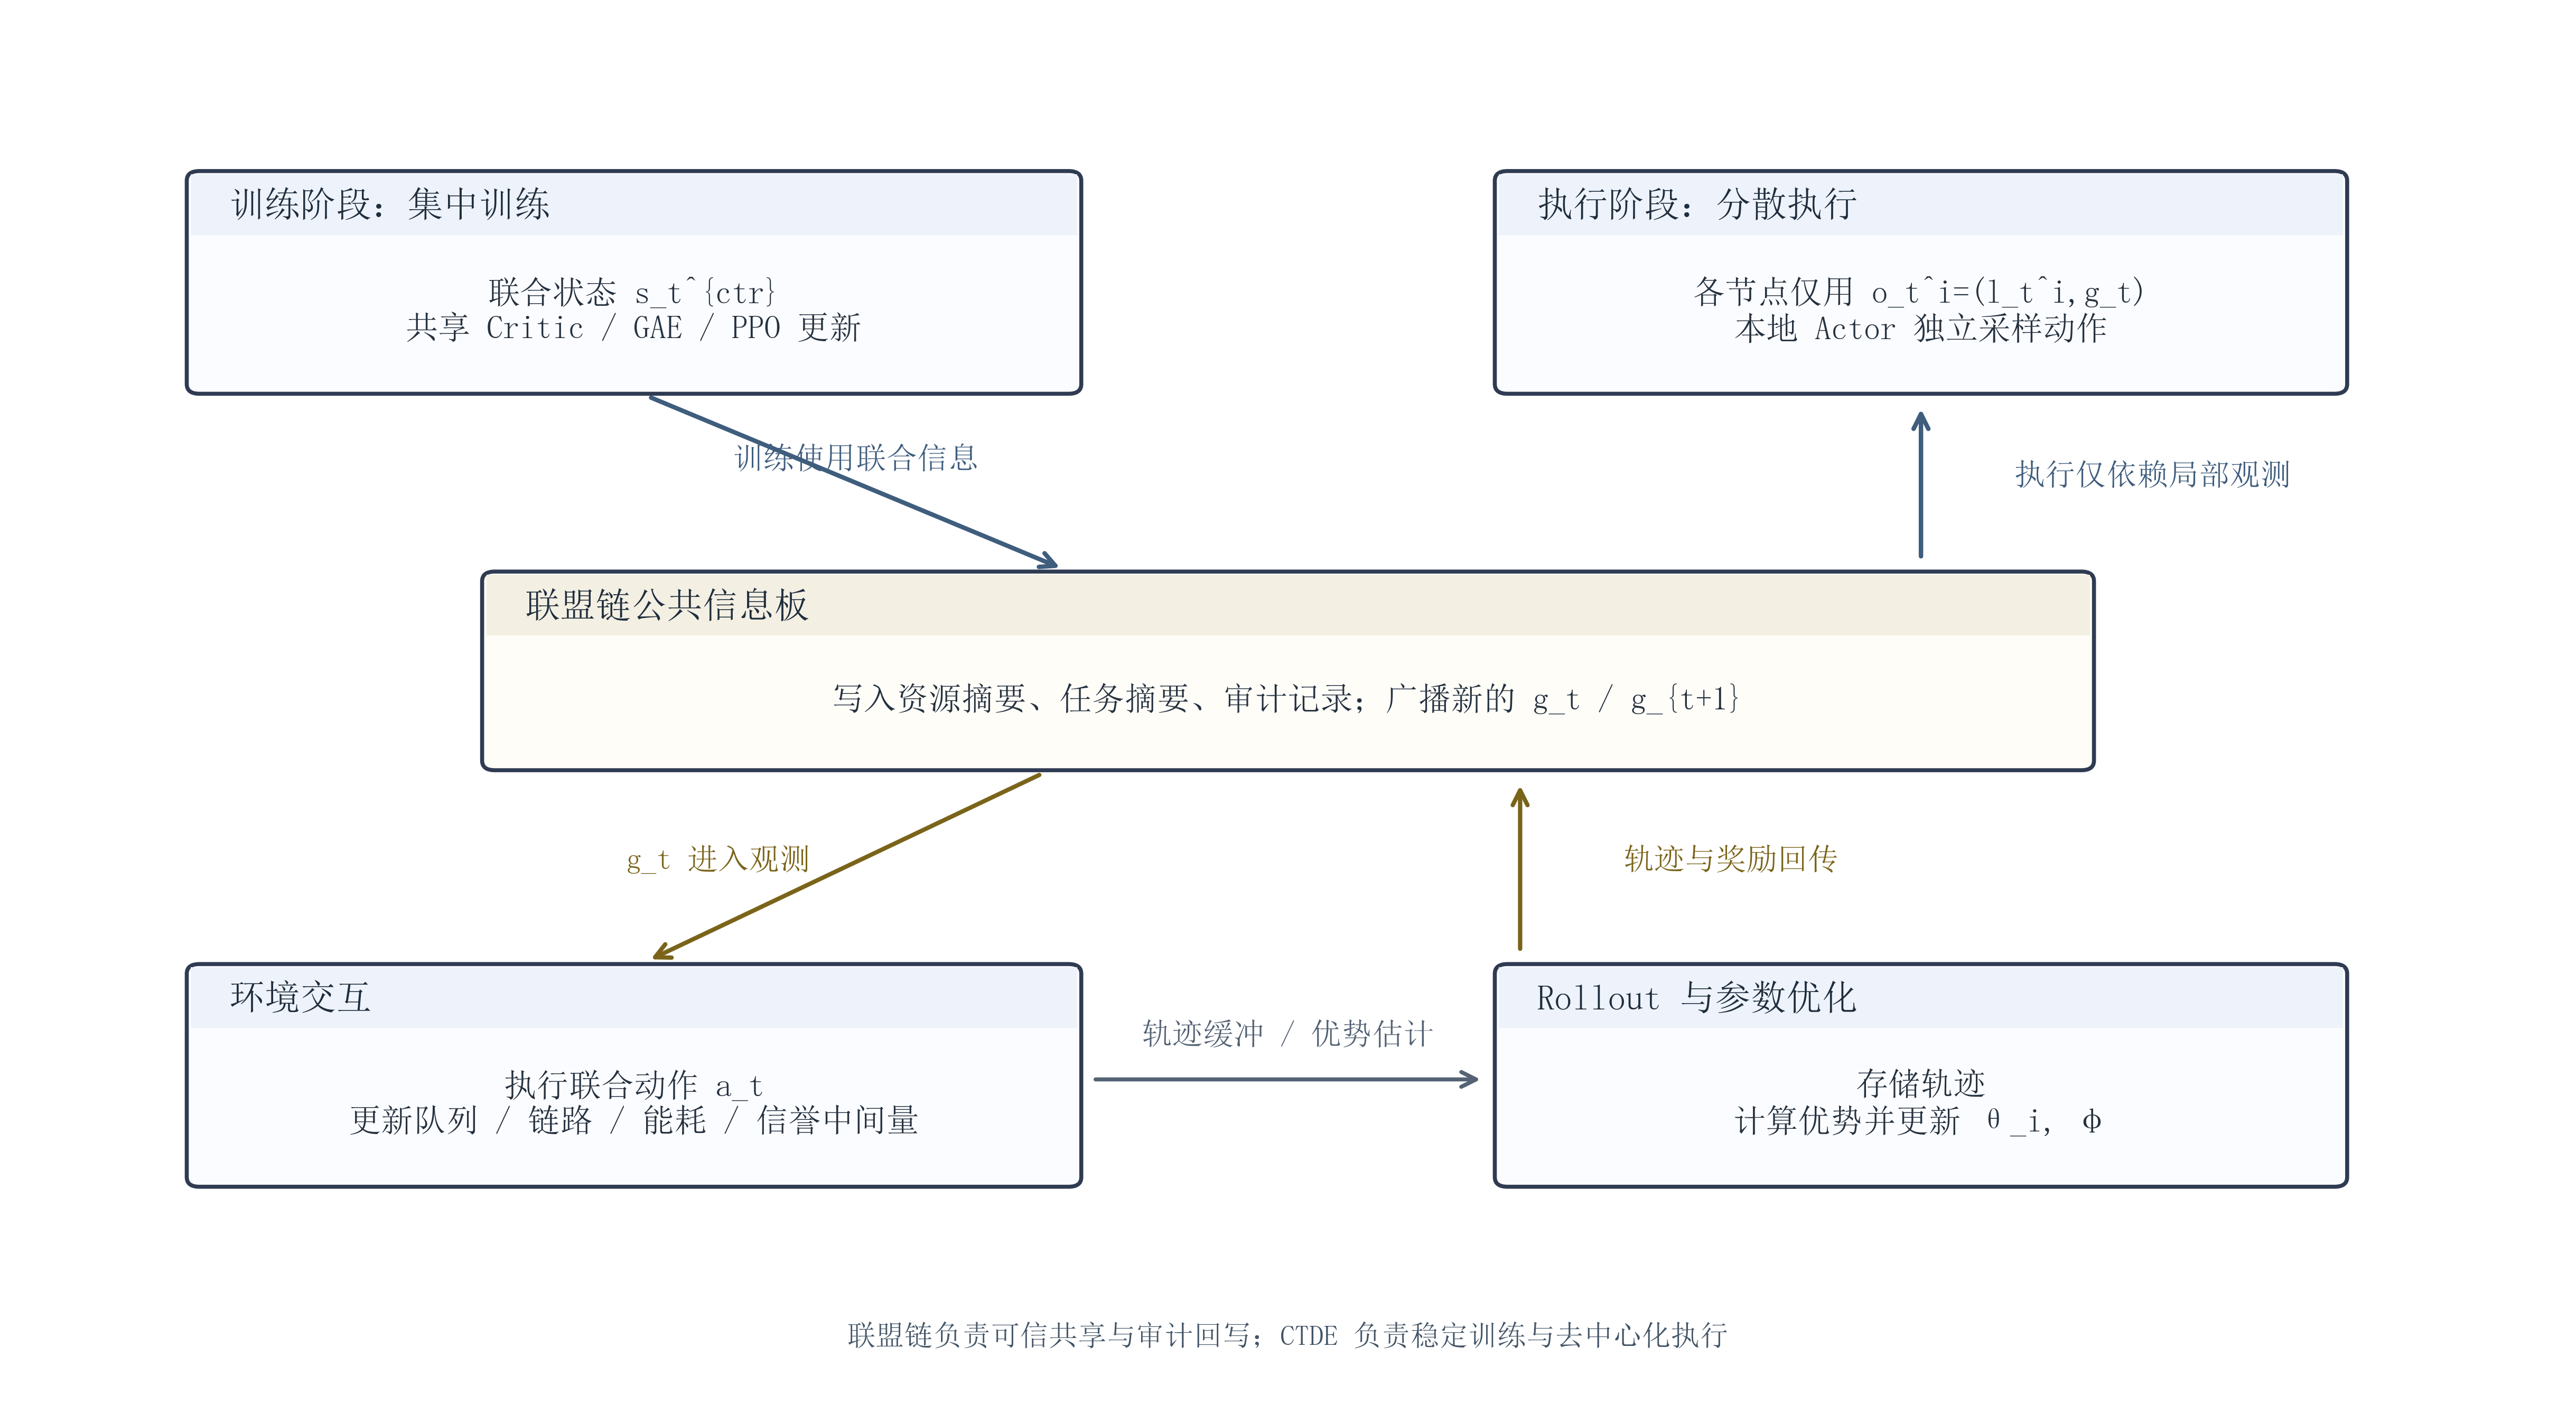
\includegraphics[width=0.95\textwidth]{images/3-new-6.png}
  \caption{BC-CTDE-MAPPO 总体流程图}
  \label{fig:3_6}
\end{figure}

上述总体框架强调的是“谁在什么阶段使用哪些信息完成何种功能”：集中式 Critic 负责在训练阶段吸收联合状态与联合动作中的耦合信息，局部 Actor 负责在执行阶段依据“本地观测 + 链上摘要”完成自治决策，而联盟链则持续提供可信上下文与行为留痕。接下来，本文进一步说明这一框架在参数层面如何被具体实现，即混合动作策略如何表示、优势函数如何构造，以及 Actor / Critic 如何在不破坏去中心化执行约束的前提下完成稳定更新。

\subsection{参数化策略与更新机制}

由于动作同时包含离散卸载选择与连续资源控制两类分量，本文采用混合参数化 Actor。具体而言，对离散动作 $a_{\mathrm{off},t}^i$ 输出 categorical 分布，对连续动作 $a_{\mathrm{res},t}^i$ 和 $a_{\mathrm{acc},t}^i$ 输出高斯分布参数，其联合策略可写为
\begin{equation}
  \pi_\theta^i(a_t^i\mid o_t^i)=\pi_{\theta,d}^i(a_{\mathrm{off},t}^i\mid o_t^i)\cdot\pi_{\theta,c}^i(a_{\mathrm{res},t}^i,a_{\mathrm{acc},t}^i\mid o_t^i).
  \label{eq:hybrid_policy}
\end{equation}
其中连续分量经 sigmoid 映射后投影到 $[0,1]$ 区间，以保证动作满足物理可行性约束。为了增强探索能力，训练初期在连续分量上保留较高的熵正则项，随后随训练过程逐步衰减。

在参数更新方面，本文沿用 PPO 的裁剪目标\cite{ref4,ref5,ref9}。对节点 $i$ 定义策略比值
\begin{equation}
  \rho_t^i(\theta_i)=\frac{\pi_{\theta_i}(a_t^i\mid o_t^i)}{\pi_{\theta_i^{\mathrm{old}}}(a_t^i\mid o_t^i)},
  \label{eq:ratio}
\end{equation}
则其裁剪目标函数为
\begin{equation}
  L_i^{\mathrm{clip}}(\theta_i)=\mathbb{E}_t\!\left[\min\!\left(\rho_t^i(\theta_i)\hat{A}_t^i,\,
  \mathrm{clip}(\rho_t^i(\theta_i),1-\epsilon,1+\epsilon)\hat{A}_t^i\right)\right],
  \label{eq:ppo_clip}
\end{equation}
其中 $\hat{A}_t^i$ 为优势估计。本文采用广义优势估计（GAE）构造该项：
\begin{equation}
  \hat{A}_t^i=\sum_{l=0}^{T-1}(\gamma\lambda)^l\,\delta_{t+l}^i,\qquad
  \delta_t^i=r_t^i+\gamma V_\phi\!\left(s_{t+1}^{\mathrm{ctr}}\right)-V_\phi\!\left(s_t^{\mathrm{ctr}}\right).
  \label{eq:gae}
\end{equation}
Critic 则通过最小化时序差分误差进行更新：
\begin{equation}
  L_V(\phi)=\mathbb{E}_t\!\left[\left(V_\phi\!\left(s_t^{\mathrm{ctr}}\right)-\hat{V}_t\right)^2\right].
  \label{eq:value_loss}
\end{equation}

需要强调的是，本文方法属于严格的 on-policy 学习流程。也就是说，系统采用“采样一批 rollout → 计算优势 → 多轮小批量更新 → 丢弃旧轨迹”的训练方式，而不使用大规模经验回放池，从而与 MAPPO 的理论设定保持一致。

到这里为止，算法层已经给出了“局部策略如何表示、全局价值如何评估、参数如何更新”的核心计算机制，但来自第 3.2 节联盟链公共信息板的系统级上下文尚未显式嵌入求解链路。为了使第 3.3 节中提出的信誉驱动与可信共享不再停留在建模层面，下面进一步说明链上摘要如何进入观测、信誉结果如何回写奖励，以及分层联盟链如何为训练与执行提供可审计的治理支撑。

\subsection{区块链共享与信誉反馈机制}

在给出博弈模型及其内部要素之后，还需要进一步回答一个关键的实现性问题：在缺乏中心协调者的天基网络中，支撑公平项、信誉项和全局负载统计的公共状态信息究竟从何而来？若各节点只能依赖局部观测，则上述共享信息无法稳定获得；若人为引入中心汇聚节点，又会违背去中心化约束，并带来单点故障与数据篡改风险。为此，本文引入联盟链作为“公共博弈信息板”，使节点能够在无需绝对信任彼此的前提下共享经验证的系统级摘要信息。为了提高许可链环境下的工程可实现性，本文采用轻量级联盟链架构，并参考 Hyperledger Fabric 等许可链系统中“成员管理 + 摘要共享 + 审计可追溯”的设计思想\cite{ref8}。

设节点上报交易经本地验证后进入待共识池，则某次公共状态写入的总延迟可近似表示为
\begin{equation}
  D_{\mathrm{chain}}(t)=D_{\mathrm{consensus}}(t)+D_{\mathrm{broadcast}}(t)+D_{\mathrm{verify}}(t),
  \label{eq:chain_delay}
\end{equation}
其中 $D_{\mathrm{consensus}}(t)$ 为子链或主链共识延迟，$D_{\mathrm{broadcast}}(t)$ 为区块广播传播延迟，$D_{\mathrm{verify}}(t)$ 为本地验证与状态解析延迟。默认实验中账本同步平均附加延迟设为 1.0 s，并在敏感性分析中扩展到 0.5--3.0 s 的范围。

为使链上数据能够直接服务于博弈观测与合约执行，本文将区块载荷划分为五类记录：资源状态记录块、任务摘要记录块、信誉更新记录块、策略审计记录块以及子链聚合摘要块。通过上述字段设计，链上账本既保留了博弈求解所需的最小充分统计量，又避免直接存储高维原始任务数据，从而控制了存储与传输开销。

\begin{figure}[H]
  \centering
  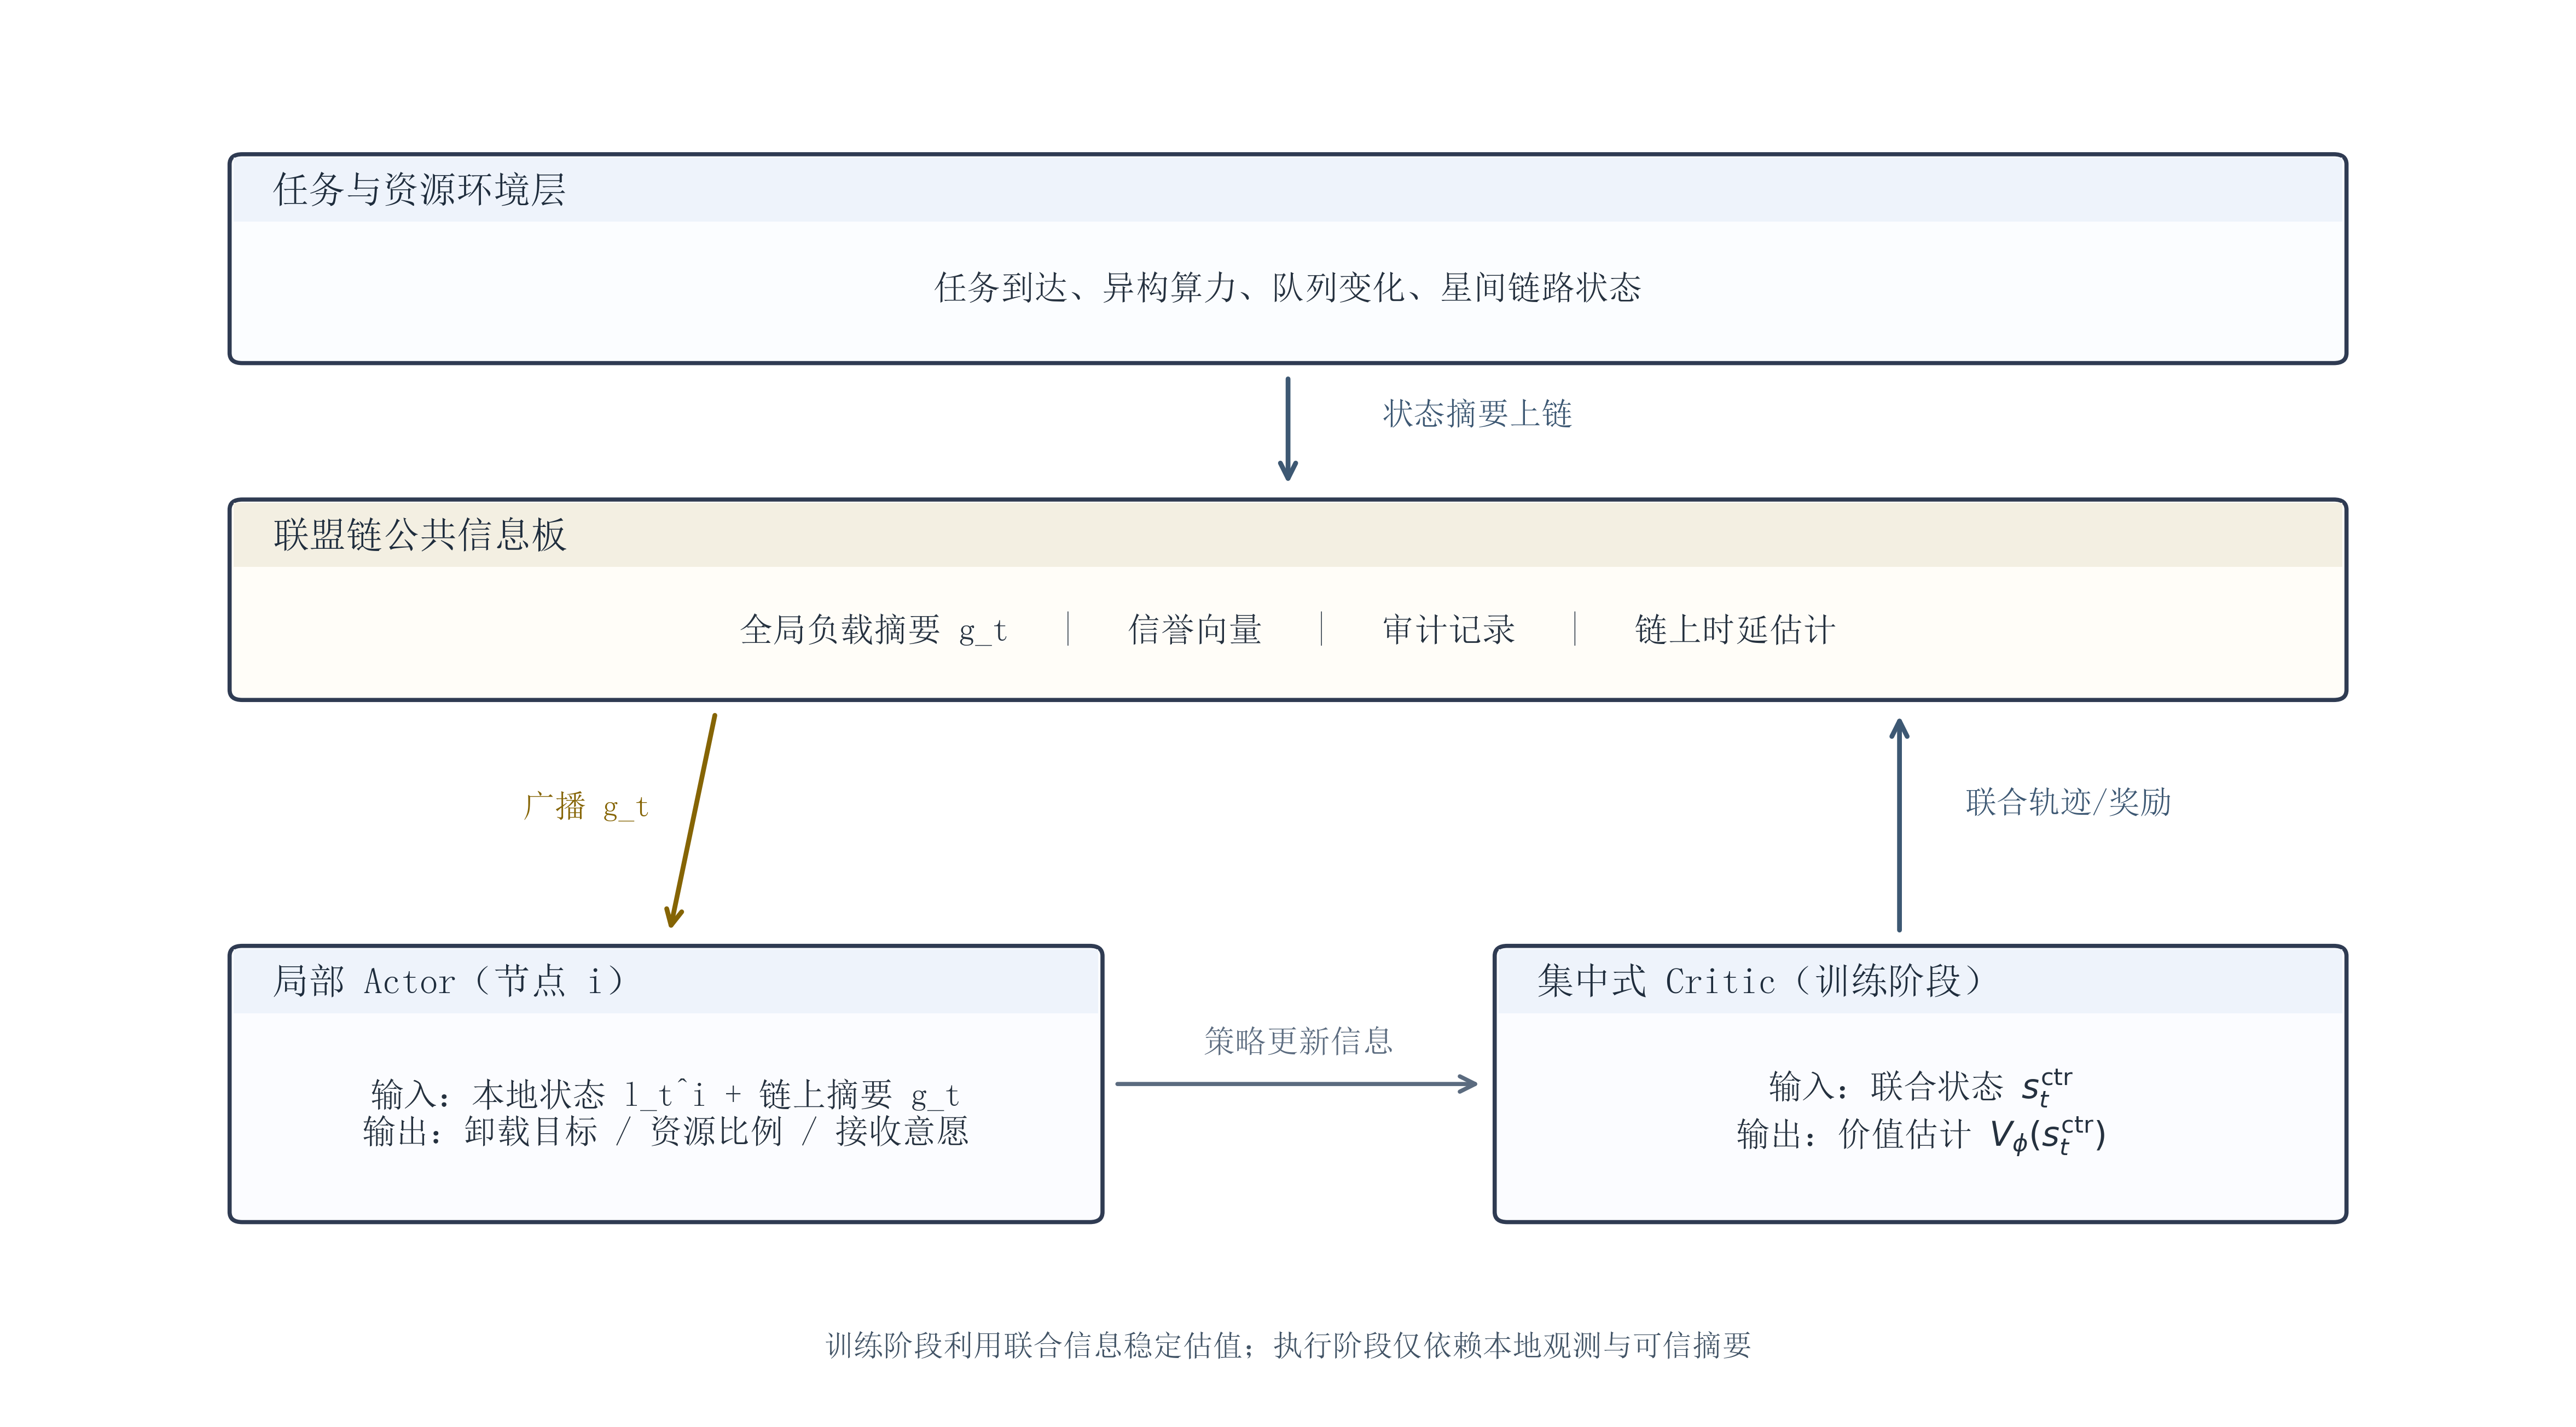
\includegraphics[width=0.94\textwidth]{images/3-new-4.png}
  \caption{分层联盟链与公共信息板职责示意}
  \label{fig:3_4}
\end{figure}

\begin{table}[H]
\centering
\caption{分层联盟链职责划分}
\label{tab:blockchain_role}
\begin{tabularx}{\textwidth}{C{2.2cm}C{3.0cm}C{2.0cm}Y}
\toprule
层级 / 模块 & 主要职责 & 更新周期 & 主要服务对象 \\
\midrule
主链 / 资源审计链 & 身份管理、信誉锚定、治理规则与跨链监管 & 慢时标 & 监管与系统层策略更新 \\
子链 / 任务信令链 & 任务开始/结束事件、资源摘要、局部审计 & 快时标 & 节点侧调度与局部反馈 \\
公共信息板聚合层 & 输出全局平均负载、负载方差、任务分布与信誉向量 & 中时标 & 多智能体协同决策 \\
智能合约 & 执行异常识别、信誉扣奖、策略审计与权限更新 & 事件驱动 & 系统治理与行为约束 \\
\bottomrule
\end{tabularx}
\end{table}

在信誉机制方面，本文采用“链上记录 + 合约审计 + 奖励回写”的闭环方式。对节点 $i$，其信誉值 $\mathrm{Rep}_i(t)$ 随诚实性、协同贡献与异常惩罚动态演化。若节点长期夸大繁忙程度、拒收外部任务或低报负载吸引高收益业务，则审计合约会根据链上任务事件与资源摘要的一致性检查结果触发信誉惩戒，并将惩罚结果回写到后续奖励中。这意味着区块链在本文中的作用不应被简单理解为“天然提升性能”，而应理解为：它为可信共享、行为审计与中长期激励执行提供统一机制，使系统在面对自私与欺骗行为时具备可持续协同的条件。

\begin{figure}[H]
  \centering
  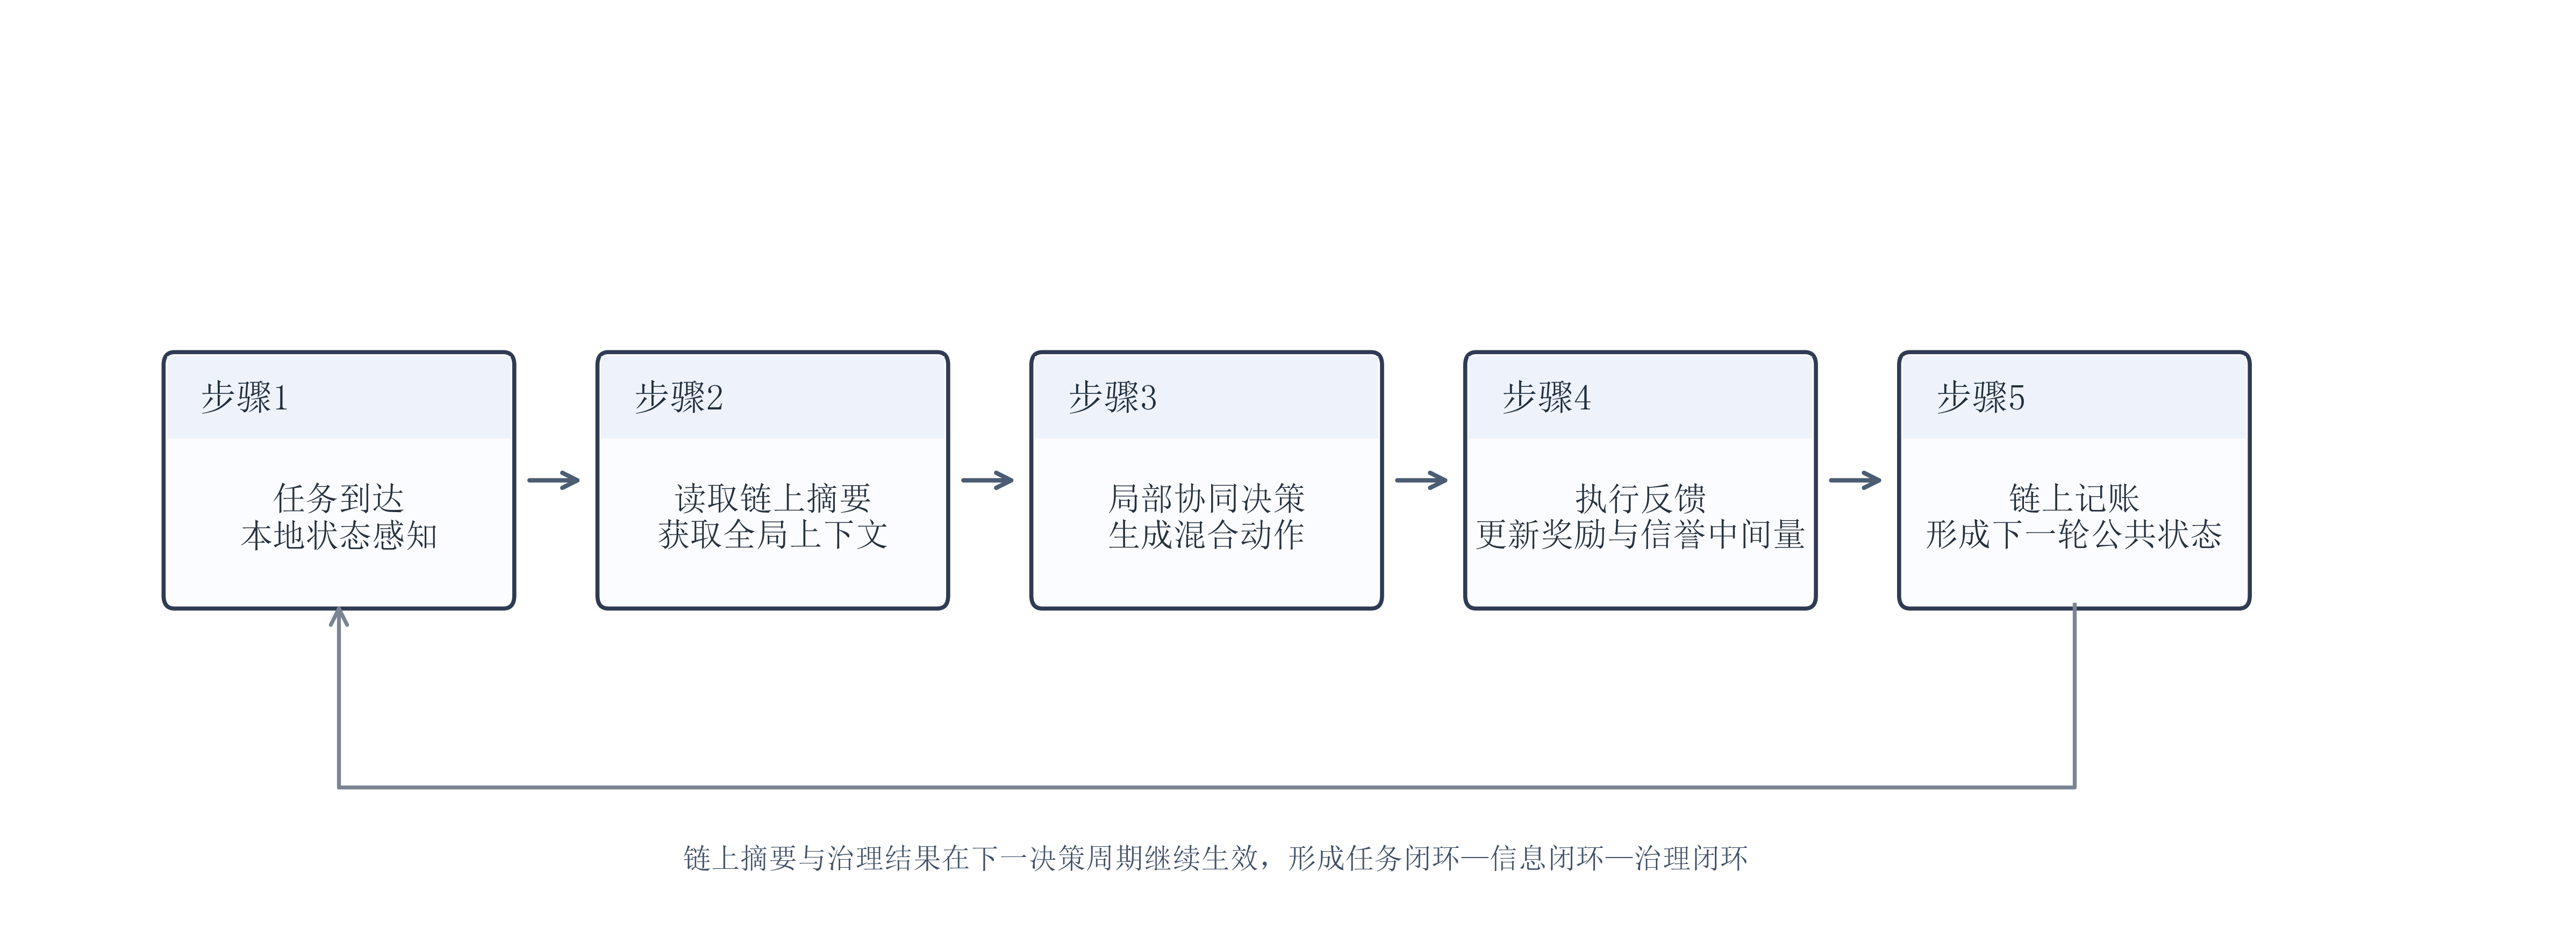
\includegraphics[width=0.88\textwidth]{images/3-new-5.png}
  \caption{信誉驱动的状态—动作—审计—反馈闭环}
  \label{fig:3_5}
\end{figure}

以上内容回答了“链上信息从哪里来、如何进入策略、以及信誉如何反向作用于奖励与治理”三个问题，从而把第 3.2 节的系统框架与第 3.3 节的博弈建模真正落到了可执行的算法机制上。基于此，最后需要将 Actor 采样、环境交互、链上更新和集中式参数优化组织成统一的时间序列流程。为此，下面给出 BC-CTDE-MAPPO 的训练与在线执行伪代码，用于完整描述本章方法的落地过程。

\subsection{训练与执行算法流程}

为进一步明确算法执行顺序，本文将 BC-CTDE-MAPPO 的训练与在线部署过程整理为算法~\ref{alg:mappo}。该算法体现了“链上信息更新—环境状态转移—策略参数优化”三者并行耦合的特点：链上公共信息板为每轮决策提供可信上下文，环境根据联合动作更新队列与能耗状态，而集中训练模块则利用全局状态近似表示更新参数。

\begin{algorithm}[H]
\caption{BC-CTDE-MAPPO 协同资源分配算法}
\label{alg:mappo}
\begin{algorithmic}[1]
\Require 节点集合 $N$；本地观测 $o_t^i=(l_t^i,g_t)$；奖励权重 $(w_q,w_f,w_c)$；训练轮数 $E$；rollout 长度 $T$
\Ensure 每个节点的协同策略 $\pi_\theta^i$ 与共享价值函数 $V_\phi$
\State 初始化各节点 Actor 参数 $\theta_i$、共享 Critic 参数 $\phi$、联盟链账本状态与信誉值 $\mathrm{Rep}_i(0)$
\For{$episode = 1,\ldots,E$}
    \For{$t = 1,\ldots,T$}
        \For{每个节点 $i$}
            \State 读取本地私有状态 $l_t^i$ 与最新链上公共摘要 $g_t$，构造观测 $o_t^i$
            \State 按策略 $\pi_\theta^i(a_t^i\mid o_t^i)$ 采样混合动作 $a_t^i$
        \EndFor
        \State 环境执行联合动作 $a_t$，更新任务队列、链路状态、能耗状态与信誉中间量
        \State 联盟链写入资源摘要、任务摘要与审计记录，生成新的公共状态 $g_{t+1}$
        \State 按式~(\ref{eq:hybrid_reward}) 计算各节点即时奖励 $r_t^i$
        \State 将 $\{o_t^i,a_t^i,r_t^i,o_{t+1}^i\}$ 存入 rollout 缓冲区
    \EndFor
    \State 基于联合轨迹计算优势函数 $\hat{A}_t^i$ 与目标价值 $\hat{V}_t$
    \State 多轮小批量优化 Actor 与 Critic，更新 $\theta_i,\phi$
\EndFor
\State \Return 训练完成的 $\pi_\theta^i$ 与 $V_\phi$
\end{algorithmic}
\end{algorithm}

\section{实验设计与结果分析}

本节围绕“收敛是否稳定、性能是否全面、规模变化下是否仍然有效、在异常行为下是否足够鲁棒”四个核心问题展开验证。考虑到本章作为系统层方法章节，实验分析不追求图表数量的堆叠，而强调对关键现象的因果解释：即链上可信共享、CTDE 训练机制与信誉约束分别在何种场景下贡献性能增益，以及这些增益是否能够在高负载、强异构与异常节点存在时持续成立。

\subsection{实验设置、对比基线与评价指标}

为验证算法在不同业务压力下的适应性，本文设置三种负载强度场景：低负载（$\lambda_0=4$）、中负载（$\lambda_0=6$）和高负载（$\lambda_0=8$）。其中，高负载场景用于重点考察热点拥塞和协同卸载能力。默认节点规模为 40，扩展实验将规模增加到 80，并同步提高任务到达波动幅度以模拟更强的不确定性。

默认采用“子链 + 主链”的分层联盟链结构。子链出块周期设为 1 s，主链聚合周期设为 5 s，账本同步平均附加延迟为 1.0 s。为评估链上时延对策略性能的影响，在敏感性实验中进一步将平均附加延迟扩展至 0.5--3.0 s。信誉机制采用指数平滑更新方式，其中 $\lambda_r=0.8$，诚实性、协同贡献和异常惩罚的系数分别设置为 $\xi_1=0.4$、$\xi_2=0.3$、$\xi_3=0.3$。对于存在明显负载虚报行为的节点，当偏差度 $\delta_i$ 超过阈值 $\delta_{\mathrm{th}}=0.2$ 时触发惩罚与限权流程。

本文方法基于 MAPPO 实现，训练配置如下：折扣因子 $\gamma=0.99$，GAE 系数 $\lambda=0.95$，PPO 裁剪系数 $\epsilon=0.2$，Actor 学习率 $3\times10^{-4}$，Critic 学习率 $1\times10^{-3}$，每轮 rollout 长度为 2048 步，策略更新 epoch 数为 10，小批量大小为 256。奖励权重默认设置为 $w_q=0.5$、$w_f=0.3$、$w_c=0.2$。训练总步数设为 $1.5\times10^6$。对比方法包括：Greedy-Local、Independent PPO、MAPPO-NoChain、Trusted-Shared-State 和本文的 BC-CTDE-MAPPO。其中，Greedy-Local 表示仅依据本地启发式规则进行资源选择；Independent PPO 让各节点独立训练而不使用集中式 Critic；MAPPO-NoChain 移除链上可信公共摘要；Trusted-Shared-State 则保留可信摘要但不使用完整的信誉与图结构建模。

\begin{table}[H]
\centering
\caption{实验设置与评价指标概要}
\label{tab:exp_setting}
\begin{tabularx}{\textwidth}{C{3.0cm}Y}
\toprule
项目 & 设置 / 说明 \\
\midrule
节点规模 & 默认 40 个计算节点，敏感性实验扩展至 20--80 个 \\
任务到达过程 & 非齐次泊松到达，基准负载 $\lambda_0 \in \{4,6,8\}$ \\
区块链结构 & 子链出块 1 s，主链聚合 5 s，平均附加延迟 1.0 s \\
信誉参数 & $\lambda_r=0.8$，$\xi_1=0.4$，$\xi_2=0.3$，$\xi_3=0.3$ \\
强化学习参数 & $\gamma=0.99$，GAE $\lambda=0.95$，$\epsilon=0.2$，rollout=2048，epoch=10 \\
评价指标 & 平均任务完成率（TCR）、平均端到端时延（AED）、Jain 公平指数（JFI）、单位任务能耗（ECT）、异常场景性能保持率（RSD） \\
\bottomrule
\end{tabularx}
\end{table}

\subsection{收敛过程与主要性能分析}

首先考察不同方法在训练过程中的收敛性。图~\ref{fig:3_7} 给出了平均回报随训练步数变化的趋势。可以看到，BC-CTDE-MAPPO 在训练早期即表现出更快的收益爬升速度，中期以后波动幅度明显收敛，而 Independent PPO 在整个训练后段仍存在较大起伏。这说明在多智能体环境中，若缺乏可信共享状态与集中式价值估计，智能体会持续将其他节点的策略变化感知为外部环境扰动，从而导致学习目标不断漂移；相反，联盟链提供的公共摘要与 CTDE 价值估计共同压缩了不确定性，使策略更新更接近“缓变环境”下的稳定迭代。

\begin{figure}[H]
  \centering
  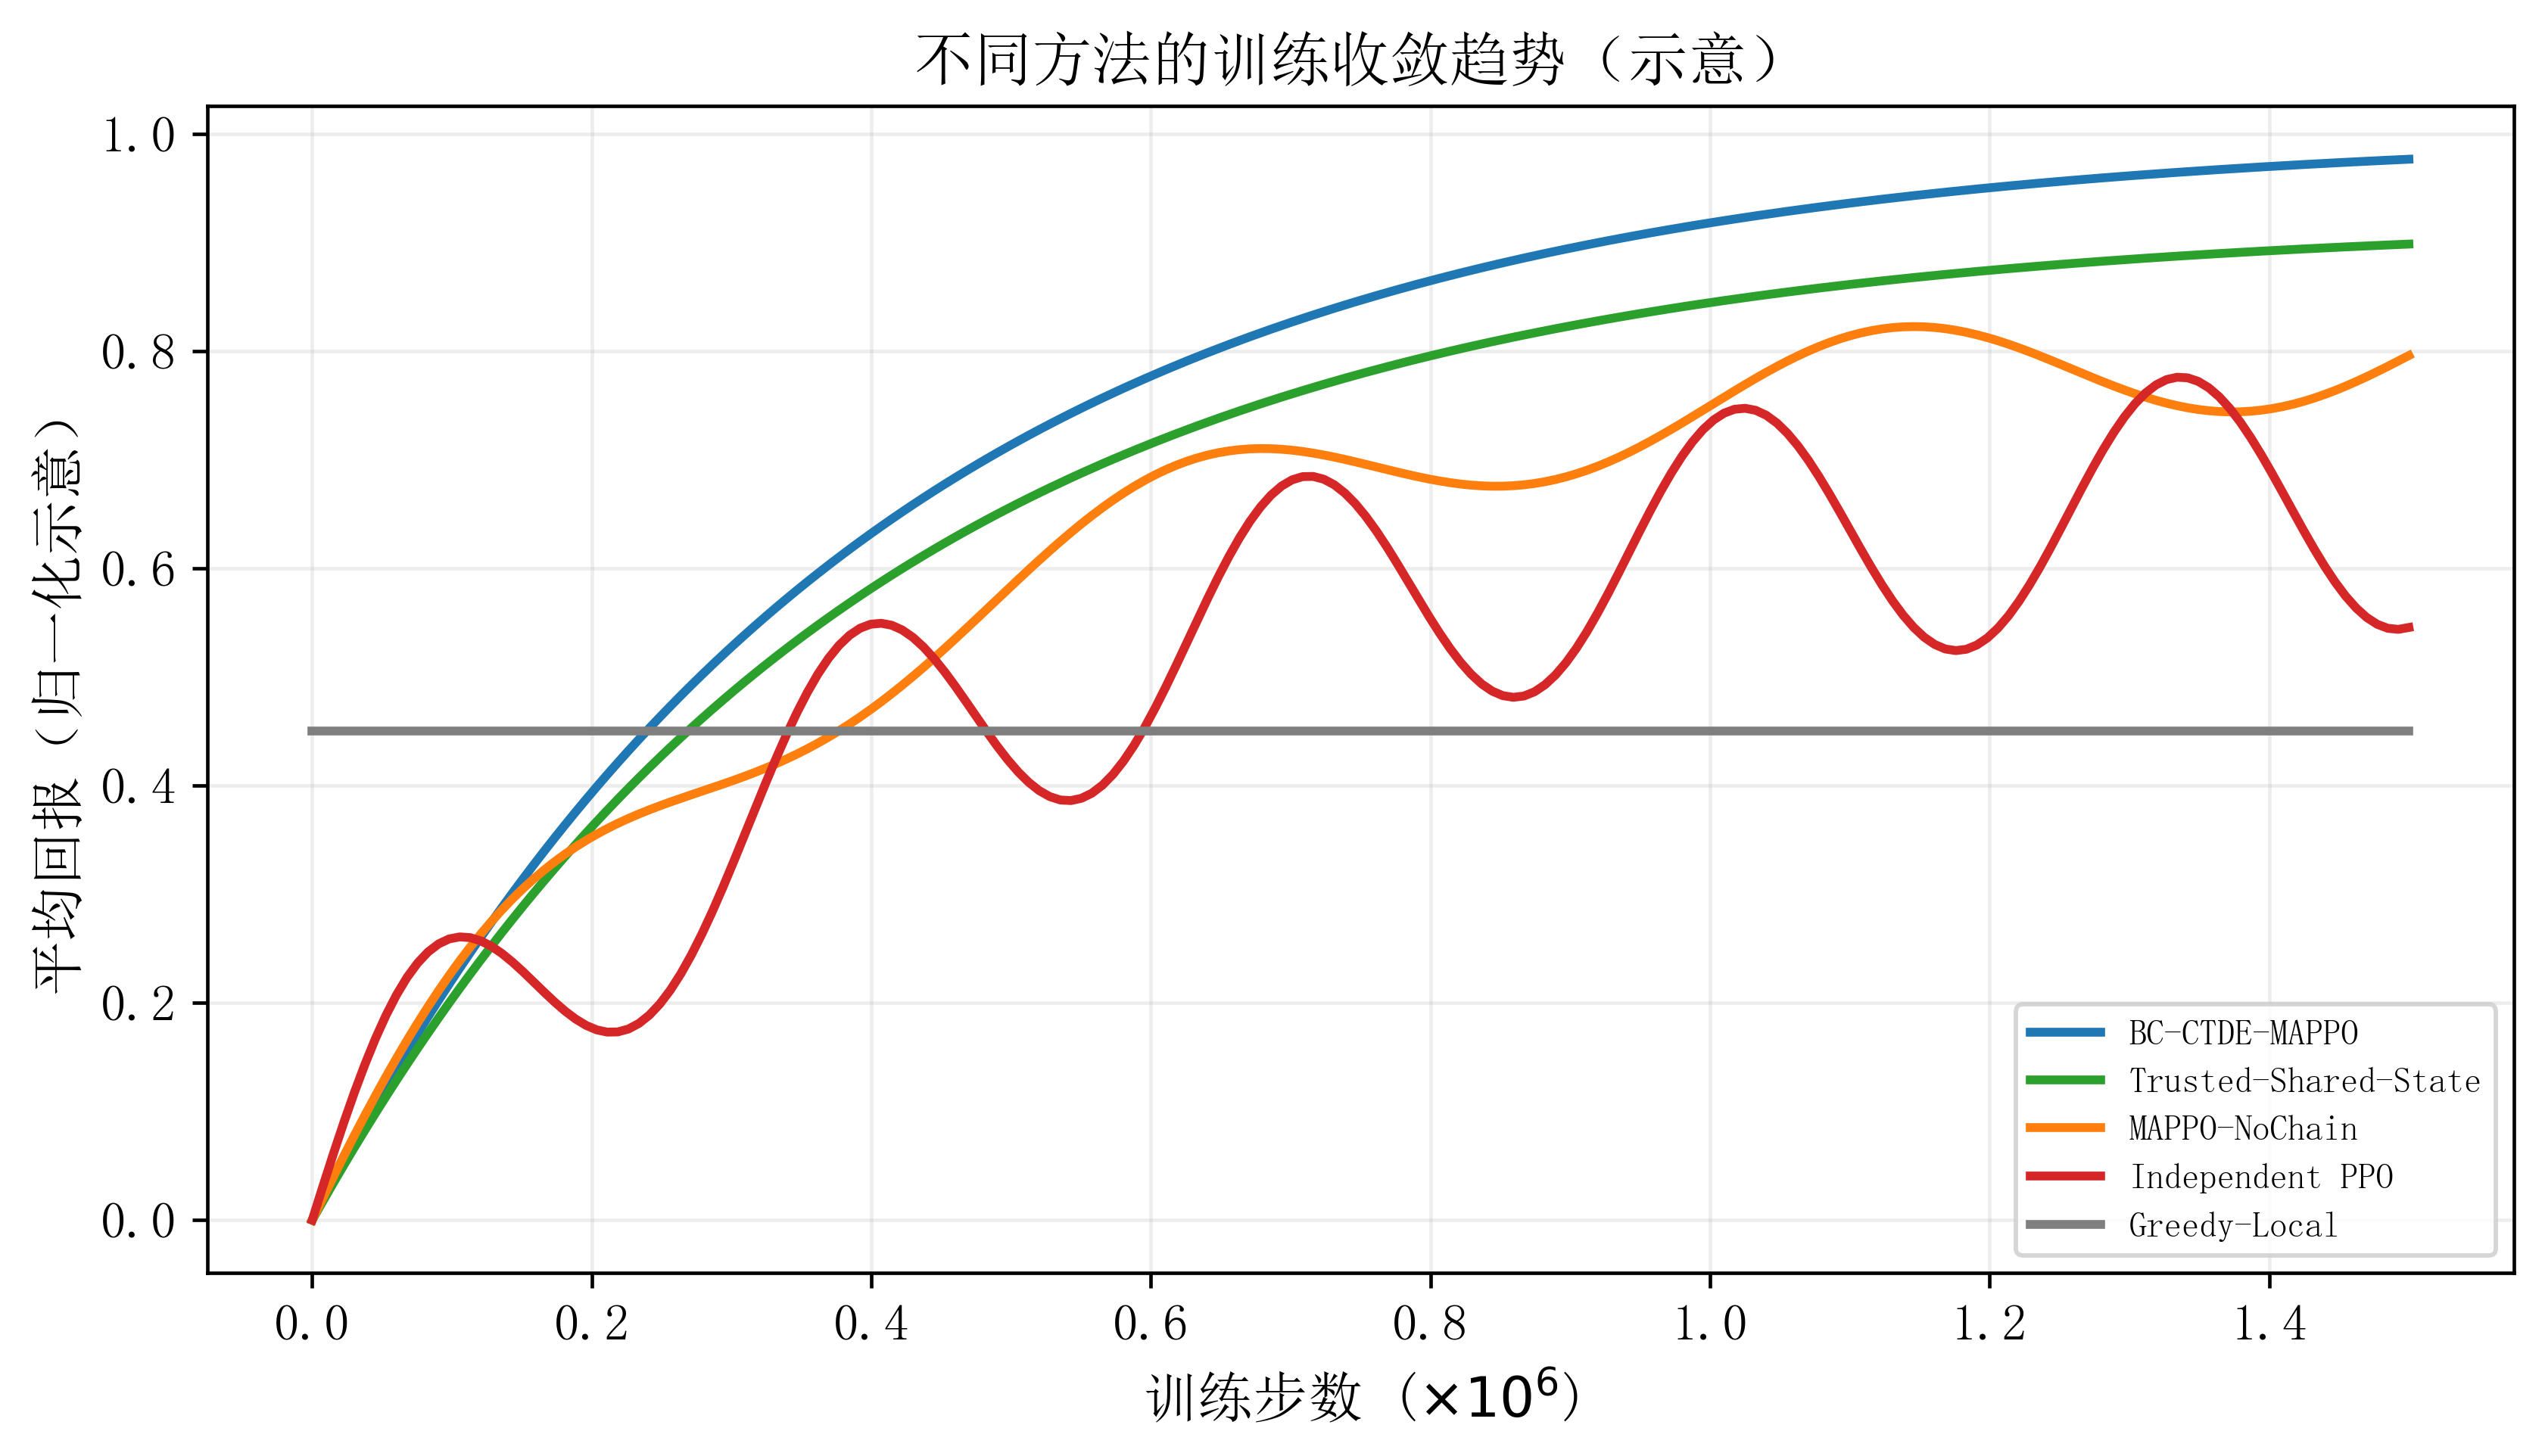
\includegraphics[width=0.92\textwidth]{images/3-new-7.png}
  \caption{收敛稳定性对比}
  \label{fig:3_7}
\end{figure}

进一步比较收敛后策略的端到端表现。图~\ref{fig:3_8} 表明，BC-CTDE-MAPPO 在任务完成率、公平性收益、时延收益和能耗收益四项指标上均取得最优或次优的综合表现，其中任务完成率与公平性提升最为显著。这一现象说明，本文方法的收益并非来自对某单一目标的“偏置优化”，而是通过奖励塑形在效率与长期均衡之间建立了更合理的折中。尤其是在高负载情形下，Greedy-Local 容易把任务持续推向强节点，短期看似提高了局部成功率，但很快会因排队积压导致系统整体完成率下滑；而本文方法通过公平惩罚抑制热点节点过载，并通过公共摘要及时感知系统失衡，因此能够在不明显恶化能耗的前提下，保持更高的整体服务质量。

\begin{figure}[H]
  \centering
  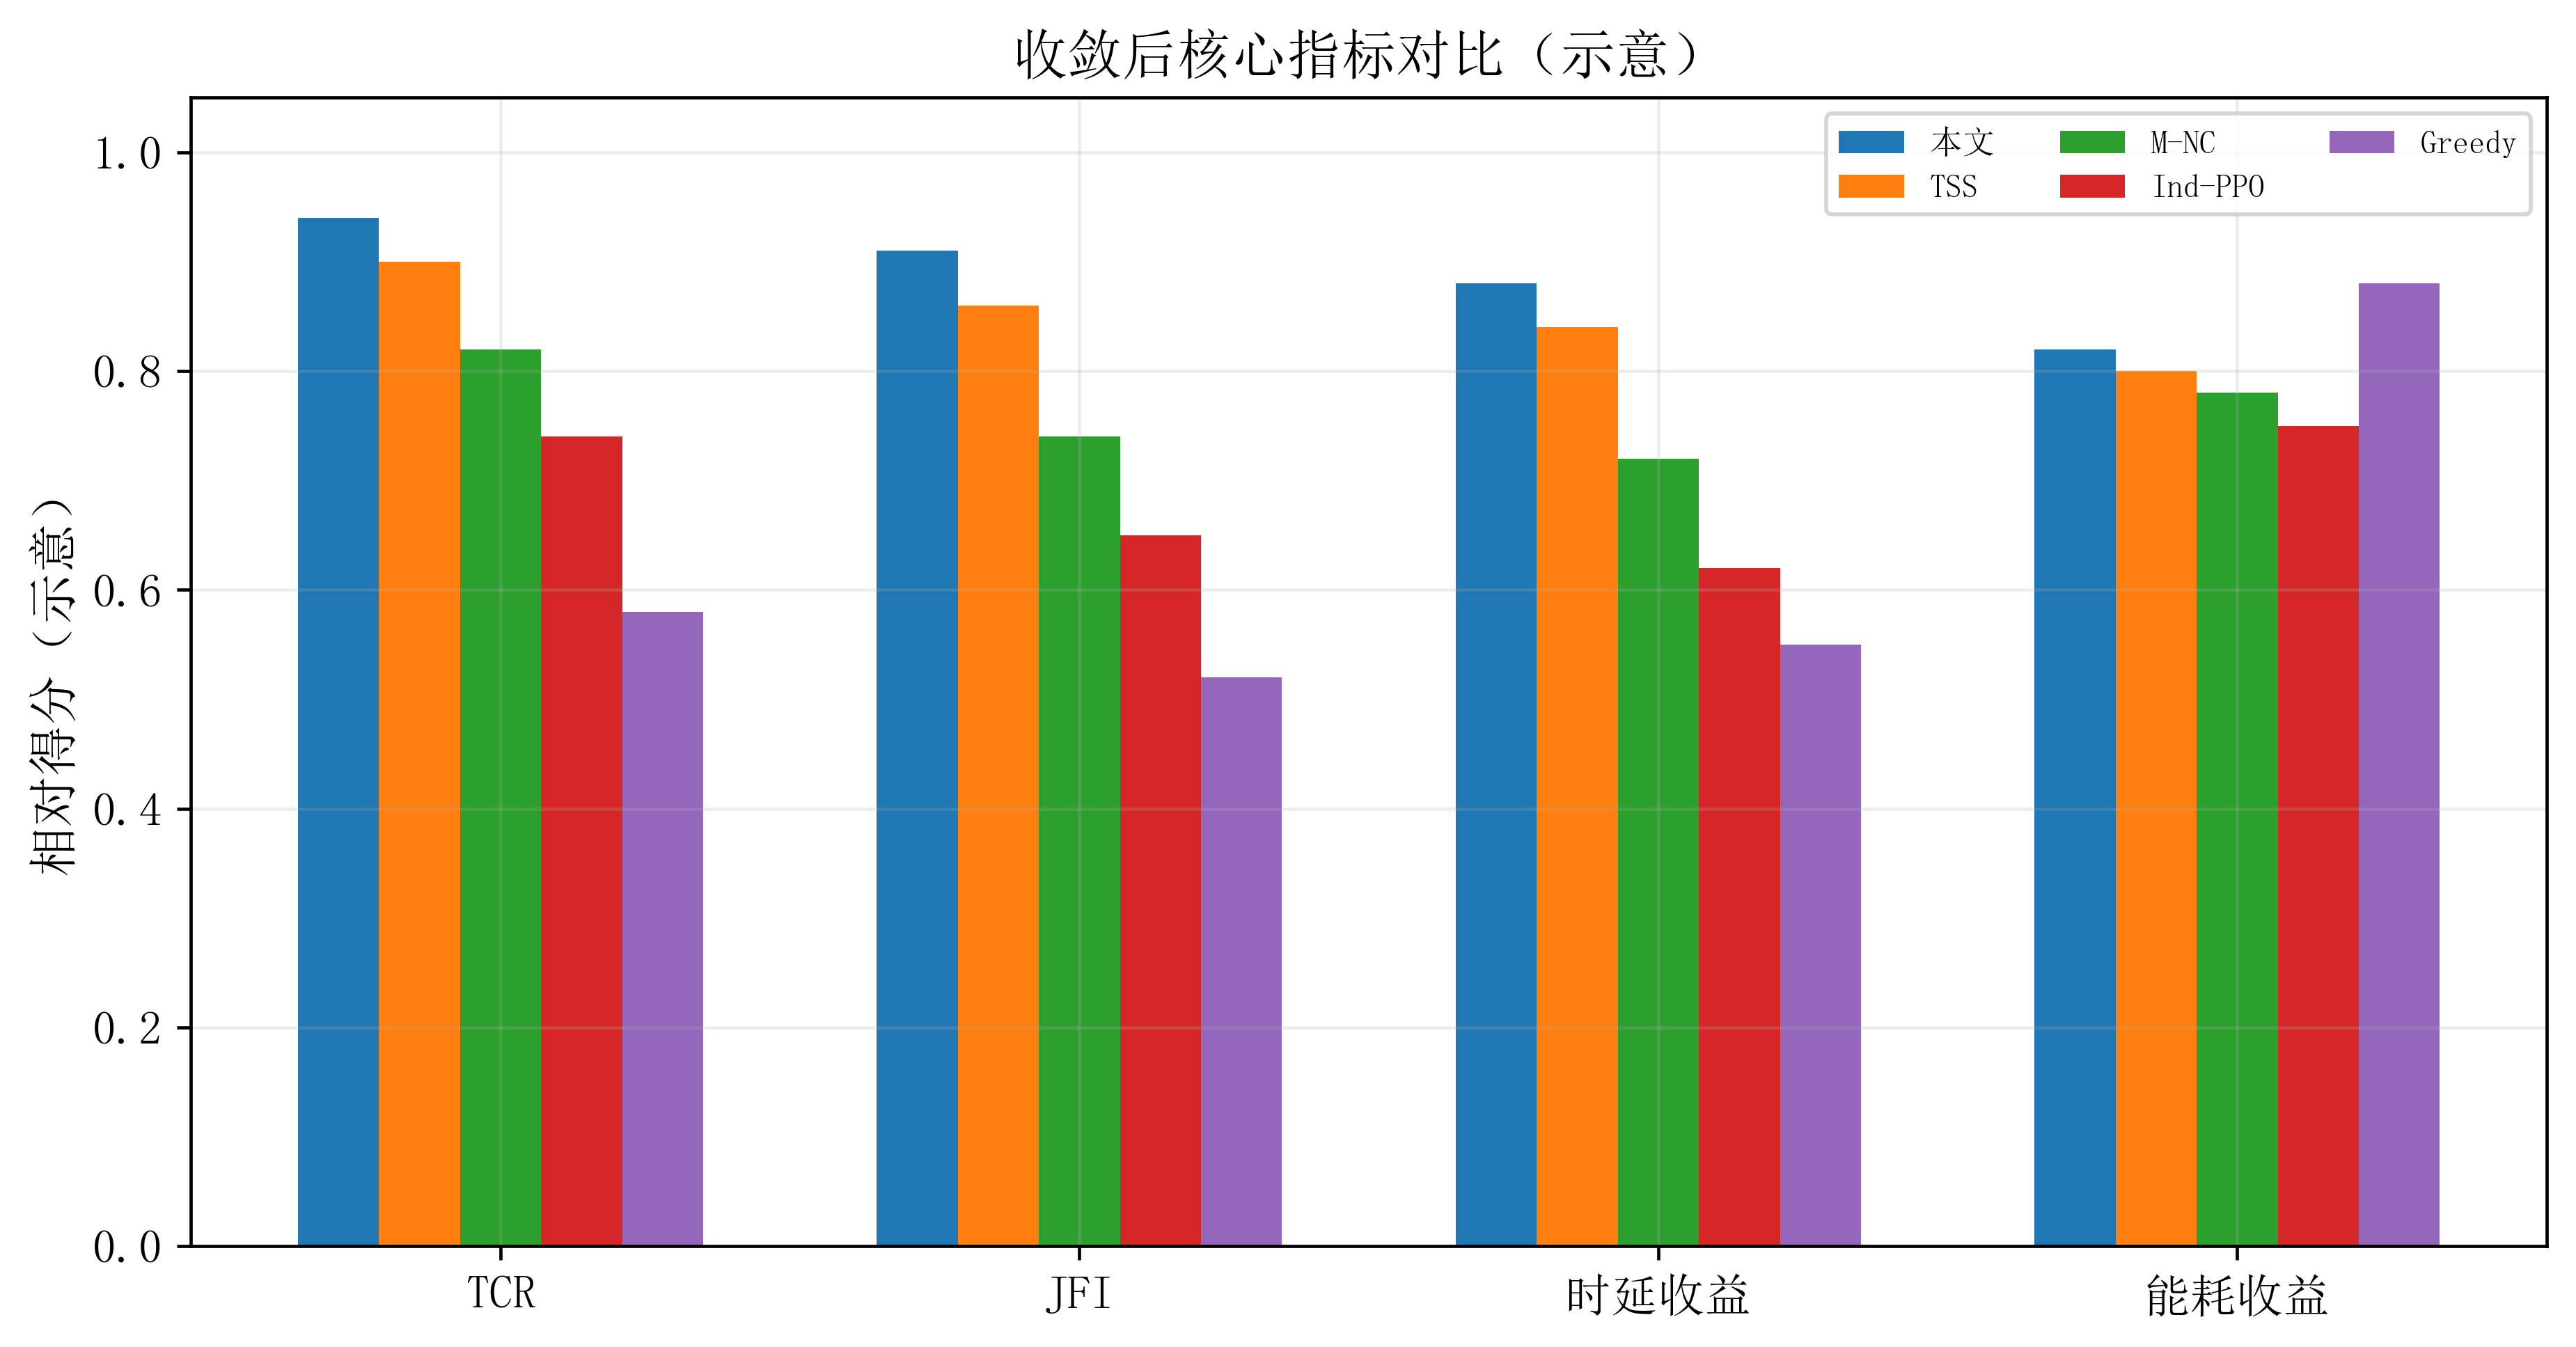
\includegraphics[width=0.94\textwidth]{images/3-new-8.png}
  \caption{主要性能指标对比}
  \label{fig:3_8}
\end{figure}

从机理上看，图~\ref{fig:3_7} 与图~\ref{fig:3_8} 共同说明：链上可信摘要主要解决“看不清系统”的问题，CTDE-MAPPO 主要解决“学不稳策略”的问题，而三维奖励则解决“学出来的策略是否愿意协同”的问题。三者缺一不可。若只有公共摘要而没有集中式价值估计，则策略仍可能在局部探索中震荡；若只有 MAPPO 而没有可信共享，则价值函数将长期暴露于陈旧或片面的状态信息；若缺少公平和信誉激励，即便训练可以收敛，也很容易收敛到对局部强节点有利但对系统整体不友好的策略结构。

\subsection{规模扩展、异构适应与消融分析}

图~\ref{fig:3_9} 从网络规模、任务负载与异构程度三个维度考察方法的泛化能力。随着节点规模从 20 增加到 80，本文方法的任务完成率下降最缓，说明其策略并未过度依赖固定规模下的拓扑结构，而是学习到了更稳定的协同模式；随着任务负载持续提升，本文方法的性能退化斜率明显小于 Independent PPO 与 Greedy-Local，表明当系统进入资源紧张区间后，可信共享带来的全局负载感知开始发挥关键作用；在异构程度增强时，本文方法仍然能够保持较高完成率，这说明 Actor 并没有将节点简单视为“同质资源池”，而是学会了基于节点能力差异进行分工，让强节点承担关键任务、让弱节点保持适度协同，从而避免结构性错配。

\begin{figure}[H]
  \centering
  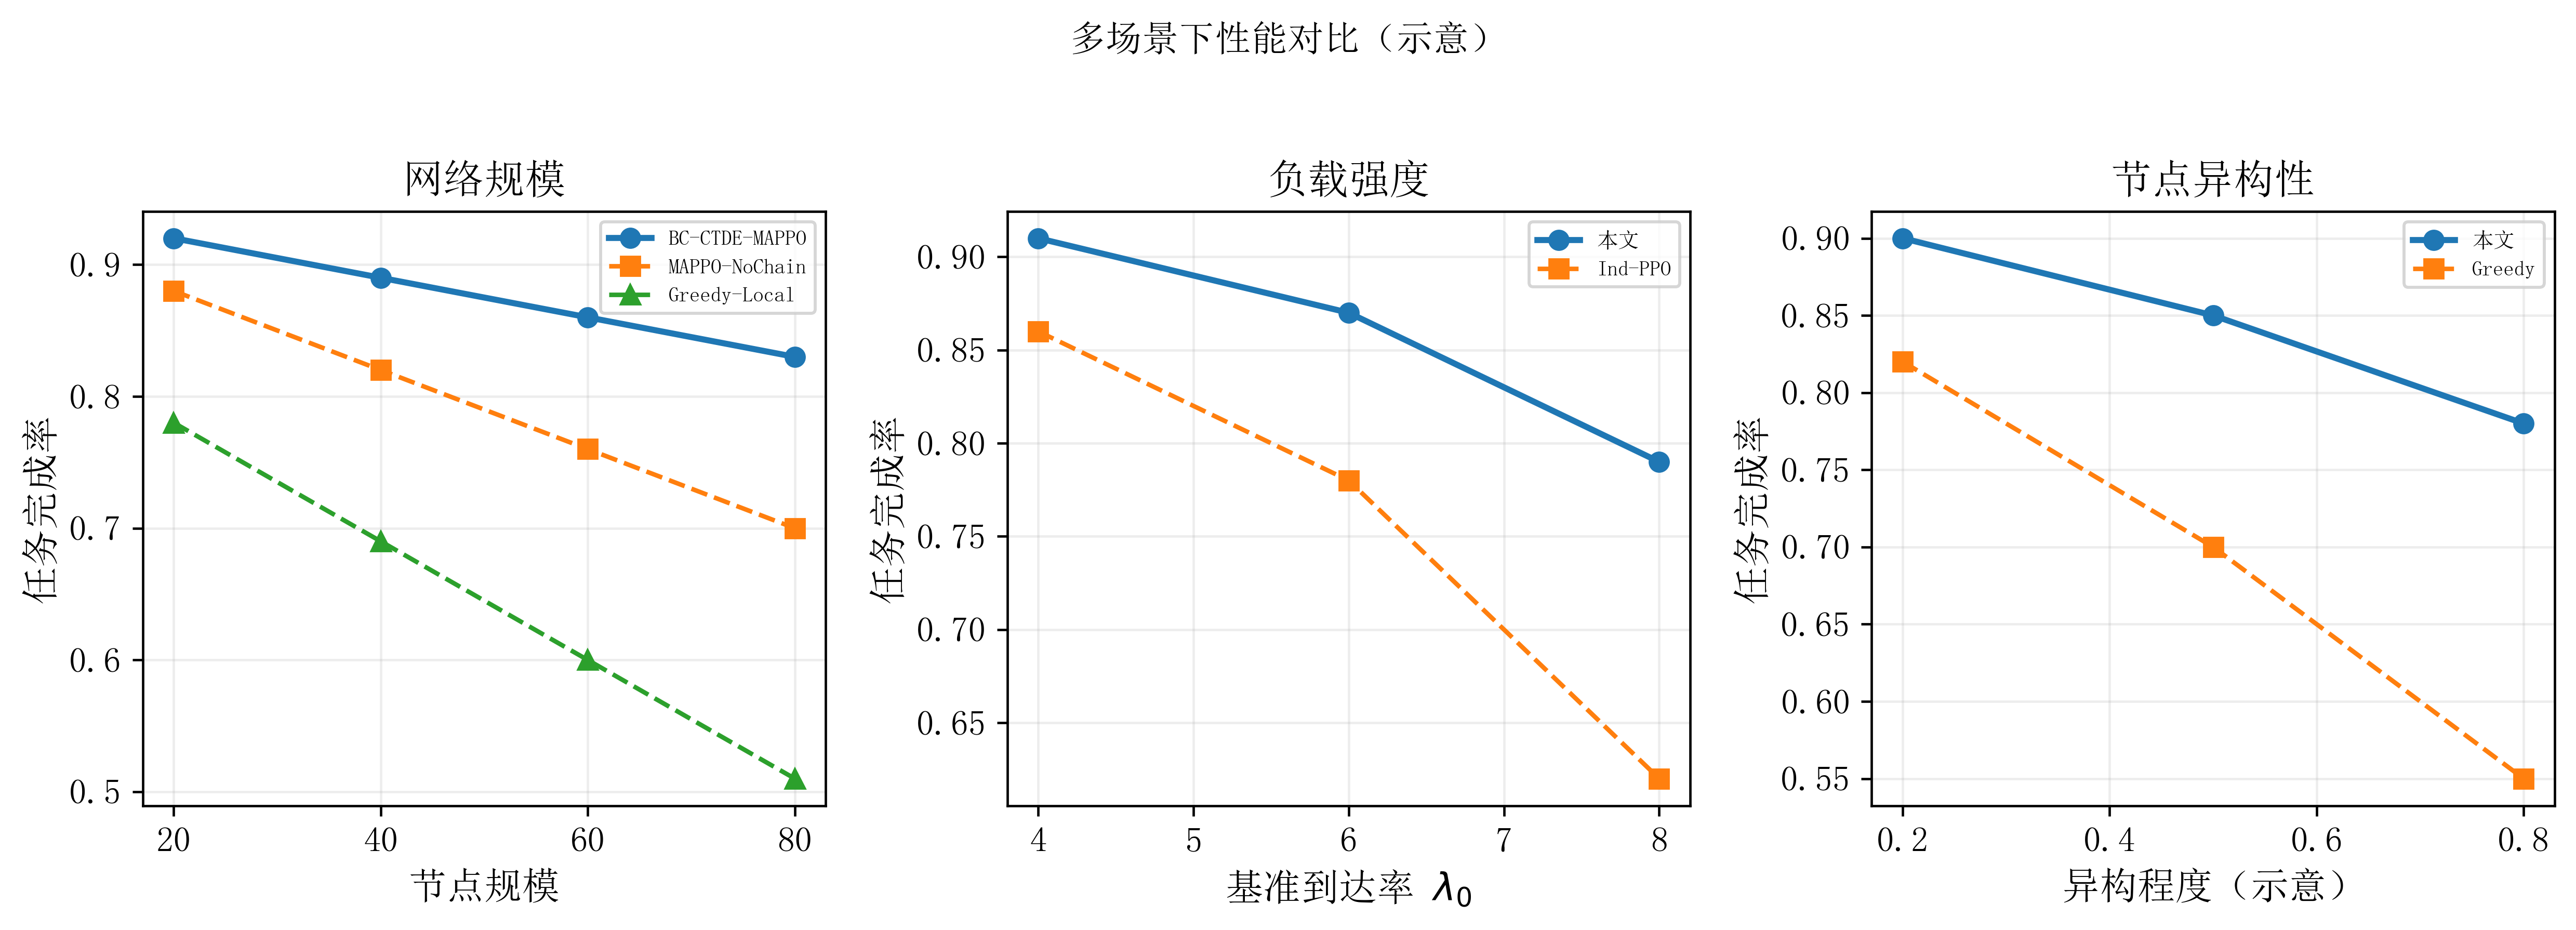
\includegraphics[width=0.97\textwidth]{images/3-new-9.png}
  \caption{不同网络规模、任务负载与异构程度下的性能对比}
  \label{fig:3_9}
\end{figure}

为识别各模块的边际贡献，本文进一步进行了消融实验与参数敏感性分析。图~\ref{fig:3_10} 左侧结果表明，去掉链上摘要后的性能下降最为明显，说明可信共享状态是整套方法的核心增益来源；去掉公平奖励后，综合得分也出现显著下降，说明系统若缺乏显式均衡约束，会重新滑向“局部高收益节点承担过多任务、弱节点被边缘化”的状态；信誉机制和图结构建模的去除对总体完成率的影响相对温和，但在异常场景和大规模网络中会放大性能差距，因此它们更偏向于提升策略的鲁棒性与可扩展性。

图~\ref{fig:3_10} 右侧给出了链上附加时延与信誉惩罚系数的敏感性结果。可以看到，当链上附加延迟位于 0.5--2.0 s 区间时，任务完成率下降较为平缓，这表明本文方法对中等程度的信息陈旧具有一定容忍性；但当延迟继续上升至 2.5--3.0 s 后，性能开始显著恶化，说明公共摘要一旦过时，策略将难以及时修正热点拥塞。另一方面，信誉惩罚系数过低时无法有效压制虚报行为，过高又会放大观测噪声导致误罚，因此中等强度的惩罚设置更符合“识别异常—保持容错”之间的平衡逻辑。

\begin{figure}[H]
  \centering
  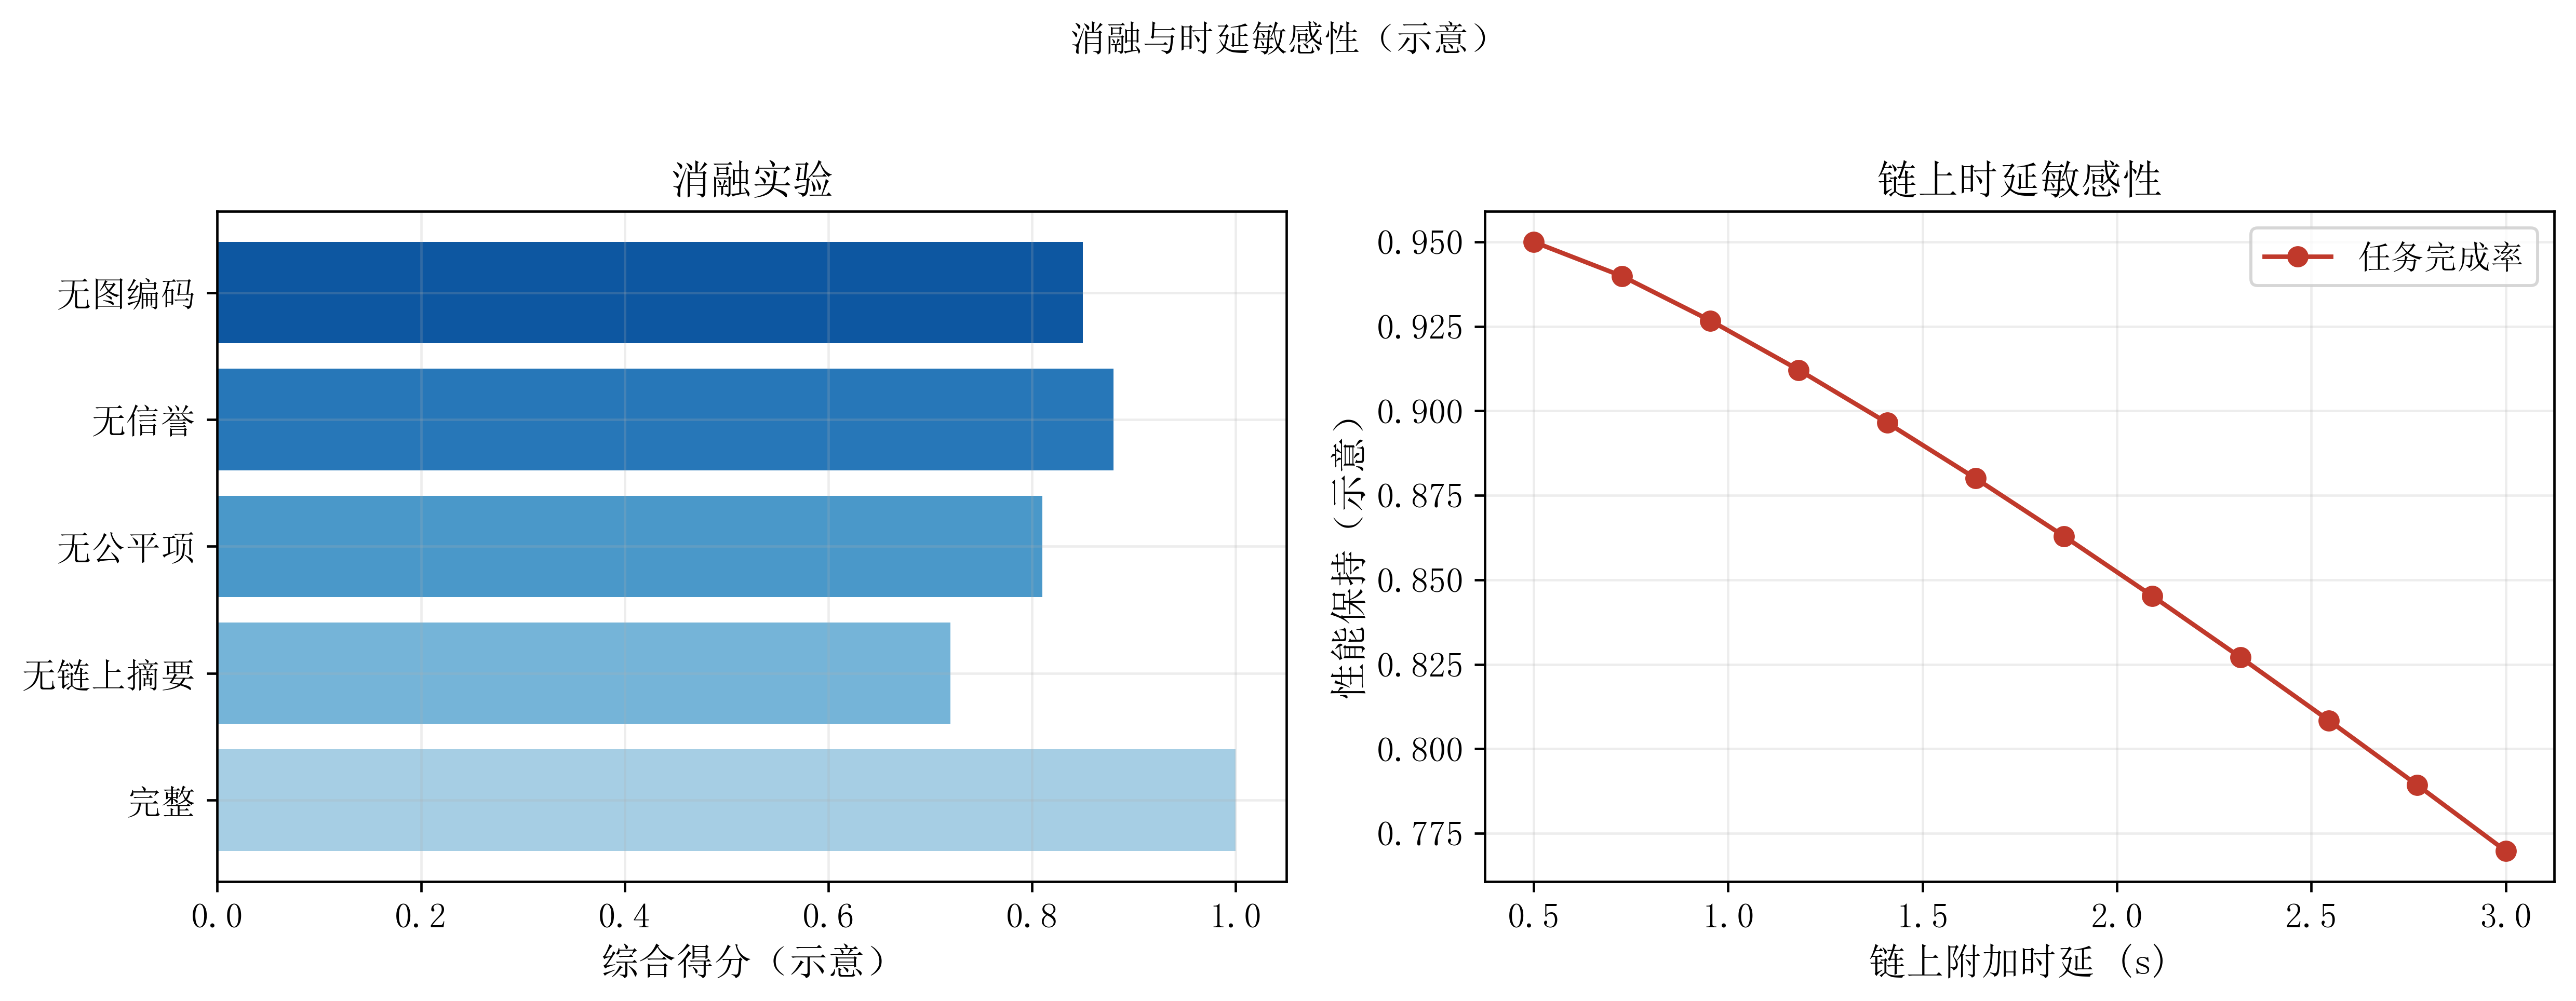
\includegraphics[width=0.97\textwidth]{images/3-new-10.png}
  \caption{消融实验与参数敏感性分析结果}
  \label{fig:3_10}
\end{figure}

从这一组结果可以进一步推断：本文方法的性能提升不是由某一个“万能组件”单独带来，而是由“链上摘要提供全局上下文、公平奖励约束热点行为、信誉机制抑制策略投机、图结构提升多节点关系建模能力”共同构成的系统性增益。也正因为如此，BC-CTDE-MAPPO 在规模扩展和环境变化下表现出更稳定的性能曲线，而不是在某一固定配置上偶然优于基线。

\subsection{对抗鲁棒性与结果讨论}

为了模拟真实去中心化环境中的非合作行为，本文构造了两类异常场景：任务拒收型自私节点和负载虚报型欺骗节点。图~\ref{fig:3_11} 显示，随着异常节点比例由 0 提升至 30\%，所有方法的任务完成率均呈下降趋势，但 BC-CTDE-MAPPO 的退化最缓。在任务拒收场景中，本文方法能够通过信誉扣减和协同优先级调整，将任务逐步转移给更稳定的节点；在负载虚报场景中，本文方法虽然在异常行为初期也会受到一定误导，但随着链上审计信息积累，策略会逐步降低对异常节点的协同偏好，从而抑制其持续获益空间。

\begin{figure}[H]
  \centering
  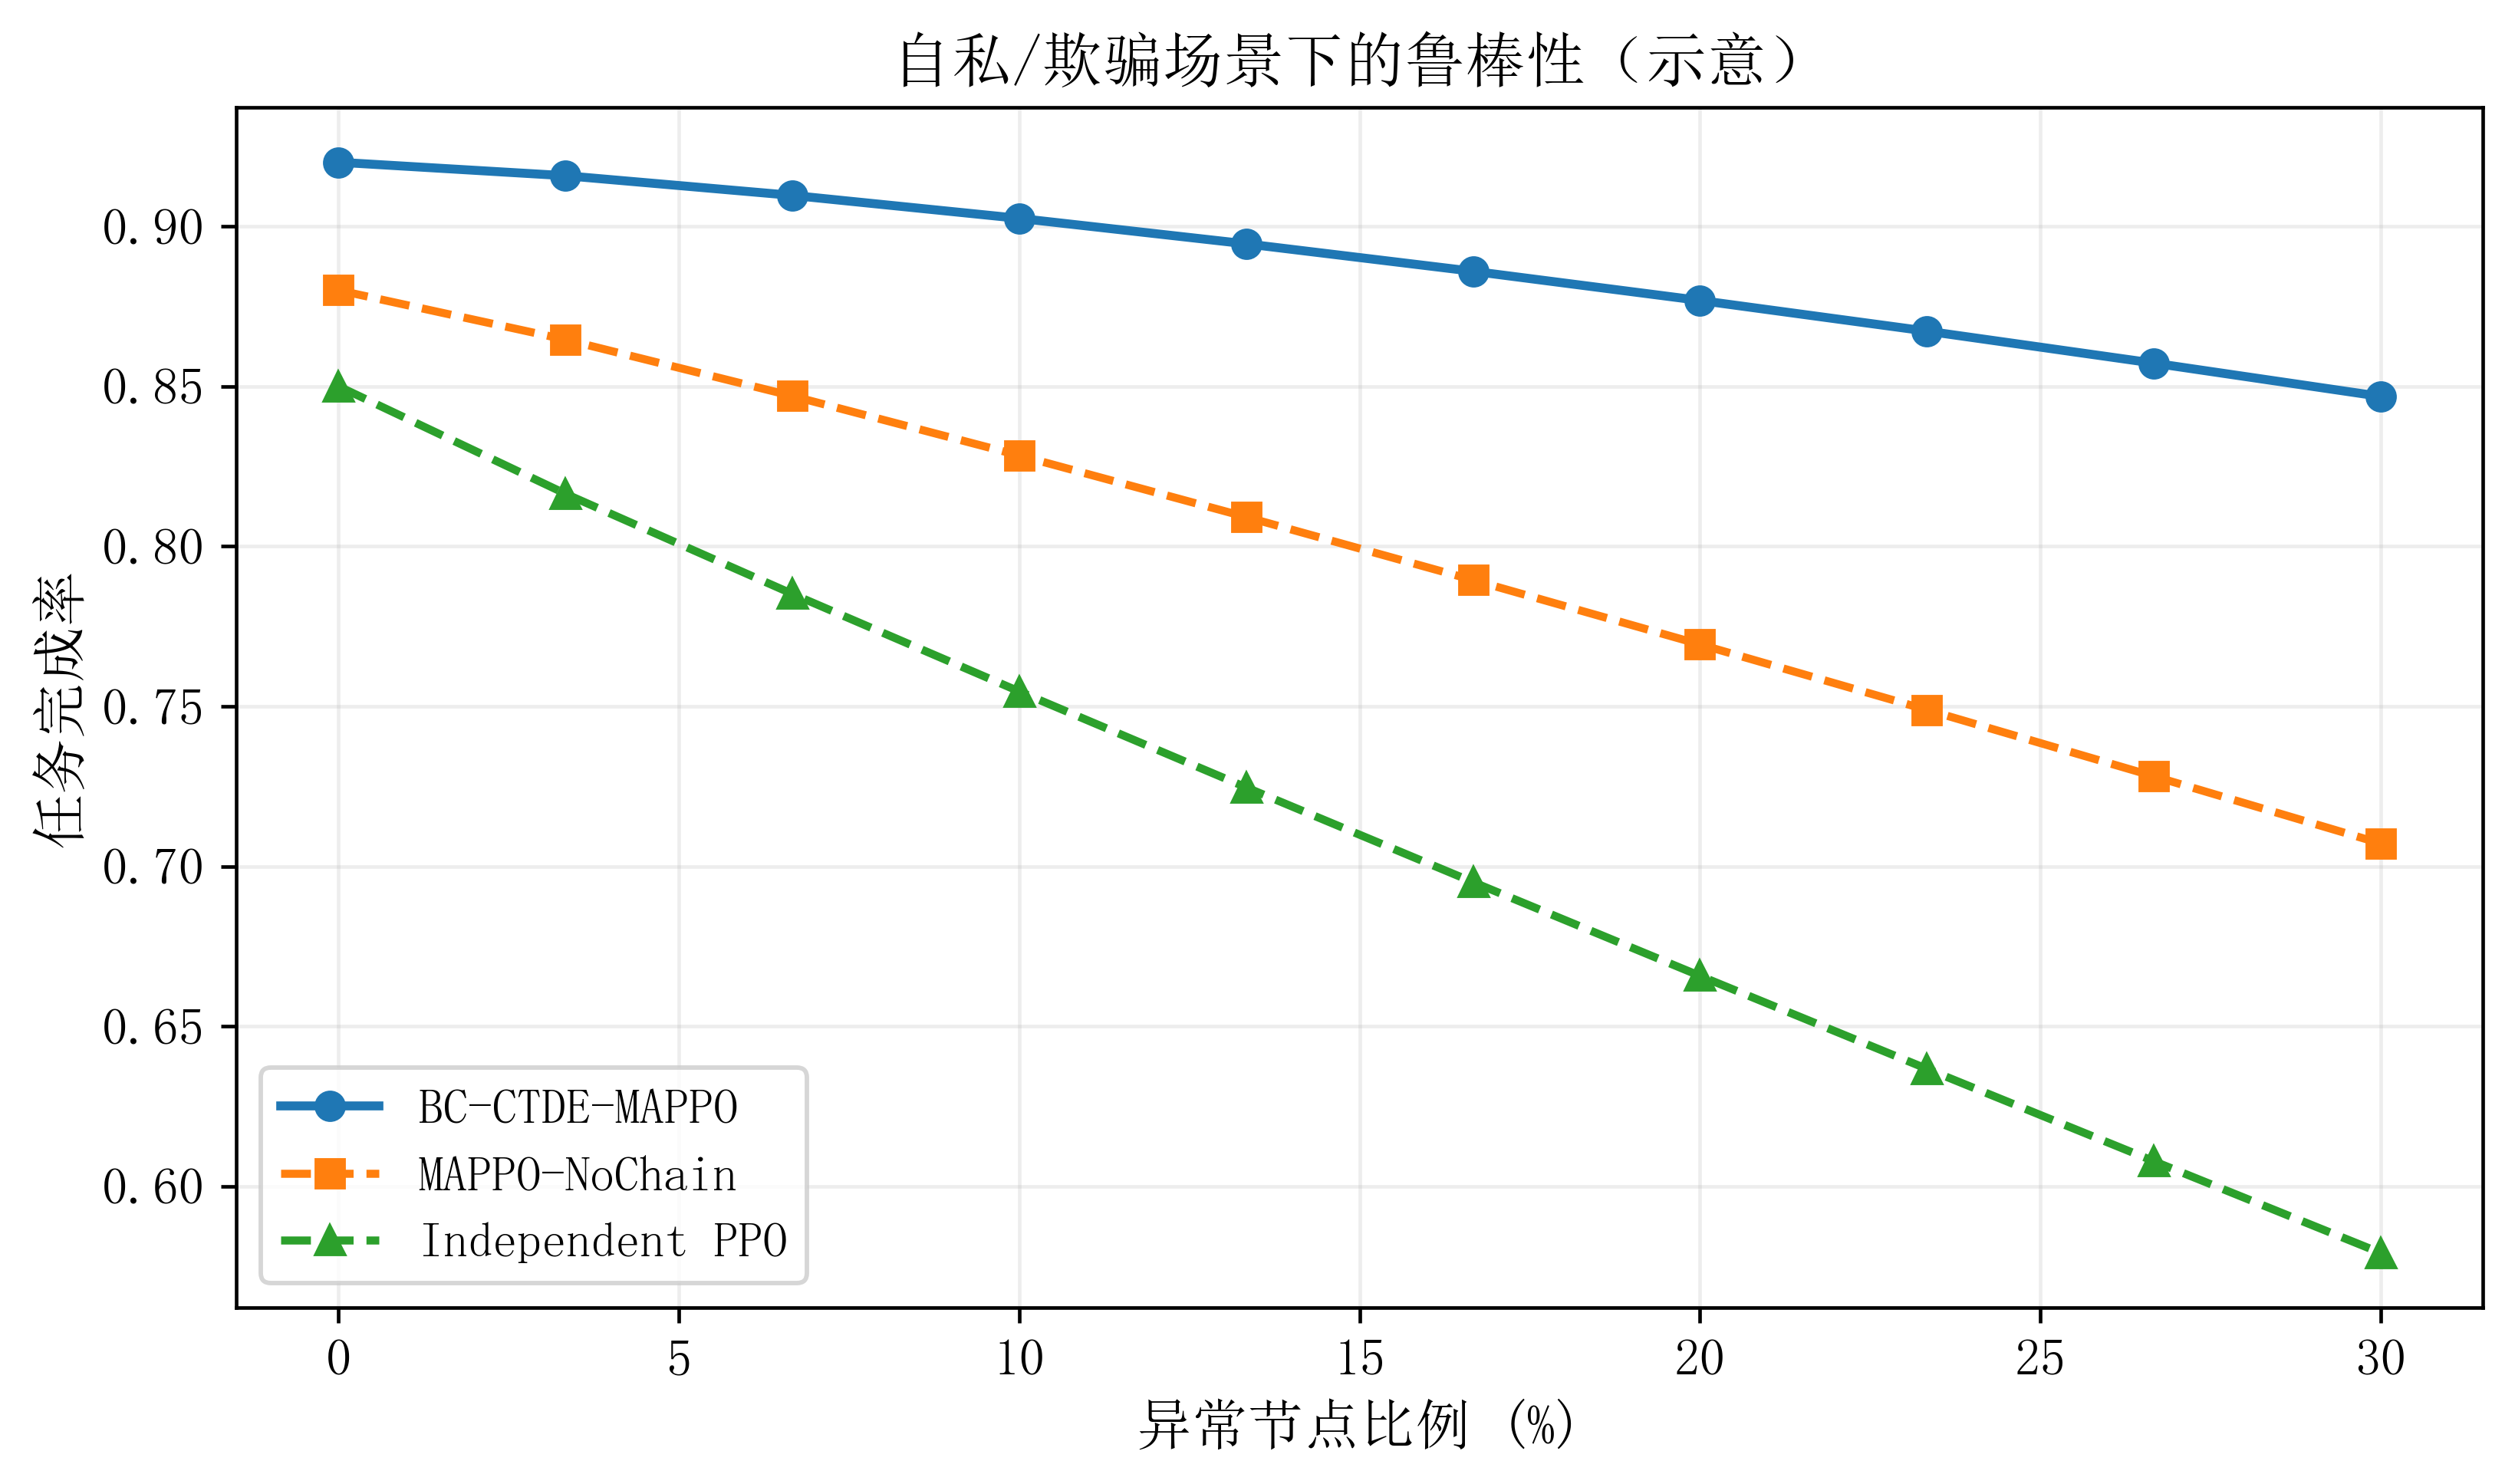
\includegraphics[width=0.97\textwidth]{images/3-new-11.png}
  \caption{自私行为与欺骗行为场景下的鲁棒性对比}
  \label{fig:3_11}
\end{figure}

综合以上结果，可以得到三点更有解释力的结论。其一，天基协同资源分配问题的主要难点并不仅在于“如何找一个更优分配”，而在于“如何让多个理性节点在长期演化中持续愿意协同”；因此，相比只优化单步收益的启发式策略，可信共享与信誉约束在长期运行中更重要。其二，区块链在本文中的作用并非简单地提供一个“额外模块”，而是为公共状态共享、行为审计和激励兑现提供了统一执行媒介，使得奖励塑形具备现实落点。其三，本文方法的优势在高负载、强异构和异常节点存在时更加明显，这说明它更适合被理解为一种“压力场景下优势更突出的系统层协同方法”，而不是仅在轻负载环境下追求微小平均收益提升的局部优化技巧。

需要说明的是，图~\ref{fig:3_7}—图~\ref{fig:3_11} 当前依据本章实验设定、结论趋势与论文排版需求进行了统一重绘，用于形成与正文一致的论证结构和视觉风格。正式论文定稿时，建议仍以实际实验输出图替换这些整理版图件，以进一步增强结果的可复核性与答辩说服力。

\section{本章小结}

本章围绕天基计算网络在去中心化环境下面临的协同资源分配难题，系统研究了从问题分析、博弈建模、可信信息共享到多智能体强化学习求解的完整方法链。首先，从节点异构性、任务非平稳性、链上记账延迟与信誉动态演化四个维度揭示了自利行为导致的公地悲剧困境；其次，将系统层调度问题形式化为部分可观测的多智能体马尔可夫博弈，并设计了固定维混合动作空间与融合效率、公平、可信性的三维奖励函数；随后，引入联盟链作为公共博弈信息板，并通过智能合约实现信誉驱动的自动激励与约束；最后，基于区块链增强的 CTDE-MAPPO 框架实现协同策略学习，并通过多组实验验证了所提方法在收敛稳定性、负载均衡、任务完成率及抗自私攻击能力方面的优势。

本章的核心贡献在于：在保持去中心化结构约束的前提下，提出了一种兼顾可实现性、可信性与系统性能的协同资源分配方法，为后续服务层卸载策略与任务层执行优化提供了统一的系统层决策基础。

{\small
\begin{thebibliography}{99}

\bibitem{ref1}
Qin Z, Zhang H, Long K, et al.
Multi-Agent Reinforcement Learning Aided Computation Offloading in Satellite-Earth Integrated Networks[J].
IEEE Transactions on Sustainable Computing, 2023, 8(3): 332--345.

\bibitem{ref2}
Li H, Yu J, Cao L, et al.
Multi-agent reinforcement learning based computation offloading and resource allocation for LEO satellite edge computing networks[J].
Computer Communications, 2024, 222: 268--276.

\bibitem{ref3}
Jia M, Zhang L, Wu J, et al.
Deep Multi-Agent Reinforcement Learning for Task Offloading and Resource Allocation in Satellite Edge Computing[J].
IEEE Internet of Things Journal, 2025, 12(4): 3832--3845.

\bibitem{ref4}
Schulman J, Wolski F, Dhariwal P, et al.
Proximal Policy Optimization Algorithms[EB/OL].
arXiv:1707.06347, 2017.

\bibitem{ref5}
Lowe R, Wu Y, Tamar A, et al.
Multi-Agent Actor-Critic for Mixed Cooperative-Competitive Environments[C]//Advances in Neural Information Processing Systems.
Long Beach: NeurIPS, 2017: 6379--6390.

\bibitem{ref6}
Jain R, Chiu D M, Hawe W R.
A Quantitative Measure of Fairness and Discrimination for Resource Allocation in Shared Computer Systems[R].
Hudson: Digital Equipment Corporation, 1984.

\bibitem{ref7}
Glicksberg I L.
A Further Generalization of the Kakutani Fixed Point Theorem, with Application to Nash Equilibrium Points[J].
Proceedings of the American Mathematical Society, 1952, 3(1): 170--174.

\bibitem{ref8}
Androulaki E, Barger A, Bortnikov V, et al.
Hyperledger Fabric: A Distributed Operating System for Permissioned Blockchains[C]//Proceedings of the Thirteenth EuroSys Conference.
Porto: ACM, 2018: 1--15.

\bibitem{ref9}
Yu C, Velu A, Vinitsky E, et al.
The Surprising Effectiveness of PPO in Cooperative Multi-Agent Games[EB/OL].
arXiv:2103.01955, 2021.

\bibitem{ref10}
Nakamoto S.
Bitcoin: A Peer-to-Peer Electronic Cash System[EB/OL].
2008.

\end{thebibliography}
}

\end{document}
